\documentclass[a4paper]{scrreprt}
\usepackage{graphicx}
\usepackage{listings}
\usepackage{color}
\usepackage{hyperref}
\usepackage{makeidx}
\usepackage{bbm}
\usepackage[super]{nth}


\usepackage{xcolor}
\usepackage{caption}
\DeclareCaptionFont{white}{\color{white}}
%\DeclareCaptionFormat{listing}{\colorbox{white}{\parbox{\textwidth}{#1#2#3}}}
%\captionsetup[lstlisting]{format=listing}
\DeclareCaptionFormat{listing}{\colorbox{gray}{\parbox{\textwidth}{#1#2#3}}}
\captionsetup[lstlisting]{format=listing,labelfont=white,textfont=white}

\lstset{ %
  language=C++,                % the language of the code
  basicstyle=\normalsize\ttfamily,           % the size of the fonts that are used for the code
%   numbers=left,                   % where to put the line-numbers
%   numberstyle=\tiny\color{gray},  % the style that is used for the line-numbers
%   stepnumber=2,                   % the step between two line-numbers. If it's 1, each line 
%                                   % will be numbered
%   numbersep=5pt,                  % how far the line-numbers are from the code
%   backgroundcolor=\color{white},      % choose the background color. You must add \usepackage{color}
%   showspaces=false,               % show spaces adding particular underscores
%   showstringspaces=false,         % underline spaces within strings
%   showtabs=false,                 % show tabs within strings adding particular underscores
%   frame=single,                   % adds a frame around the code
%   rulecolor=\color{black},        % if not set, the frame-color may be changed on line-breaks within not-black text (e.g. commens (green here))
%   tabsize=2,                      % sets default tabsize to 2 spaces
%   captionpos=b,                   % sets the caption-position to bottom
%   breaklines=true,                % sets automatic line breaking
%   breakatwhitespace=false,        % sets if automatic breaks should only happen at whitespace
%   title=\lstname,                   % show the filename of files included with \lstinputlisting;
%                                   % also try caption instead of title
%   keywordstyle=\color{blue},          % keyword style
%   commentstyle=\color{dkgreen},       % comment style
%   stringstyle=\color{mauve},         % string literal style
%   escapeinside={\%*}{*)},            % if you want to add a comment within your code
%   morekeywords={*,...}               % if you want to add more keywords to the set
}

\usepackage{amsmath}
\usepackage{empheq}

\makeindex

\newcommand{\phFac}[1]{\mathrm{e}^{\mathrm{i} #1}}
\newcommand{\phFacneg}[1]{\mathrm{e}^{-\mathrm{i} #1}}
\newcommand{\planew}[2]{\mathrm{e}^{\mathrm{i} \mathbf{#1} \mathbf{#2}}}
\newcommand{\planewneg}[2]{\mathrm{e}^{-\mathrm{i} \mathbf{#1} \mathbf{#2}}}
\newcommand{\blf}[3]{\mathbf{#1}_{#2 \mathbf{#3}}}
\newcommand{\blfs}[3]{#1_{#2 \mathbf{#3}}}
\newcommand{\vp}[1]{\mathbf{#1}_{\mathcal{\parallel}}}
\newcommand{\ve}[1]{\mathbf{#1}}
\newcommand{\pd}[1]{\frac{\partial}{\partial #1}}
\newcommand{\scalProd}[2]{\langle #1 | #2 \rangle}
\newcommand{\bra}[1]{\langle #1 |}
\newcommand{\ket}[1]{|#1 \rangle}
\newcommand{\ann}[2]{#1^{\phantom{\dagger}}_{#2}}
\newcommand{\cre}[2]{#1^\dagger_{#2}}
\newcommand{\ud}{^{\phantom{\dagger}}}
\newcommand{\dd}{_{\phantom{\dagger}}}

\begin{document}

\title{Integrid}
\subtitle{A highly versatile integration grid library for C++}
\author{Tobias Stollenwerk}
\maketitle

\tableofcontents

% % From now on put page enumeration into topline
% \pagestyle{headings}



%%%%%%%%%%%%%%%%%%%%%%%%%%%%%%%%%%%%%%%%%%%%%%%%%%%%%%%%%%%%%%%%%%%%%%%%%%%%%%%%%%%%%%%%%%%%%%%%%%%%%%%%%%%%%%%%%%%
%%%%%%%%%%%%%%%%%%%%%%%%%%%%%%%%%%%%%%%%%%%%%%%%%%%%%%%%%%%%%%%%%%%%%%%%%%%%%%%%%%%%%%%%%%%%%%%%%%%%%%%%%%%%%%%%%%%
%%%%%%%%%%%%%%%%%%%%%%%%%%%%%%%%%%%%%%%%%%%%%%%%%%%%%%%%%%%%%%%%%%%%%%%%%%%%%%%%%%%%%%%%%%%%%%%%%%%%%%%%%%%%%%%%%%%
%%%%%%%%%%%%%%%%%%%%%%%%%%%%%%%%%%%%%%%%%%%%%%%%%%%%%%%%%%%%%%%%%%%%%%%%%%%%%%%%%%%%%%%%%%%%%%%%%%%%%%%%%%%%%%%%%%%
%%%%%%%%%%%%%%%%%%%%%%%%%%%%%%%%%%%%%%%%%%%%%%%%%%%%%%%%%%%%%%%%%%%%%%%%%%%%%%%%%%%%%%%%%%%%%%%%%%%%%%%%%%%%%%%%%%%
%%%%%%%%%%%%%%%%%%%%%%%%%%%%%%%%%%%%%%%%%%%%%%%%%%%%%%%%%%%%%%%%%%%%%%%%%%%%%%%%%%%%%%%%%%%%%%%%%%%%%%%%%%%%%%%%%%%
%%%%%%%%%%%%%%%%%%%%%%%%%%%%%%%%%%%%%%%%%%%%%%%%%%%%%%%%%%%%%%%%%%%%%%%%%%%%%%%%%%%%%%%%%%%%%%%%%%%%%%%%%%%%%%%%%%%
\chapter{Introduction}

The integrid library contains highly versatile integration grid classes for \texttt{C++}. The most important one is the multigrid class. It features the integration of multiple grid regions in order to resolve sharp peaks or steps in the integrand function. Hereby one can choose between equidistant, tangential and logarithmically dense grid regions. Although the number of grid regions is not bounded, there is an index function which analytically calculates the inverse of the grid and is useful for fast interpolation purposes. Intersection and overlap of different grid region is possible and will be dealt with by favoring the better resolved grid region.

The original purpose of the multigrid class was to resolve a lot of sharp Lorentz-like peaks in a self-consistent calculation on strongly correlated electron systems.


%%%%%%%%%%%%%%%%%%%%%%%%%%%%%%%%%%%%%%%%%%%%%%%%%%%%%%%%%%%%%%%%%%%%%%%%%%%%%%%%%%%%%%%%%%%%%%%%%%%%%%%%%%%%%%%%%%%
%%%%%%%%%%%%%%%%%%%%%%%%%%%%%%%%%%%%%%%%%%%%%%%%%%%%%%%%%%%%%%%%%%%%%%%%%%%%%%%%%%%%%%%%%%%%%%%%%%%%%%%%%%%%%%%%%%%
%%%%%%%%%%%%%%%%%%%%%%%%%%%%%%%%%%%%%%%%%%%%%%%%%%%%%%%%%%%%%%%%%%%%%%%%%%%%%%%%%%%%%%%%%%%%%%%%%%%%%%%%%%%%%%%%%%%
%%%%%%%%%%%%%%%%%%%%%%%%%%%%%%%%%%%%%%%%%%%%%%%%%%%%%%%%%%%%%%%%%%%%%%%%%%%%%%%%%%%%%%%%%%%%%%%%%%%%%%%%%%%%%%%%%%%
%%%%%%%%%%%%%%%%%%%%%%%%%%%%%%%%%%%%%%%%%%%%%%%%%%%%%%%%%%%%%%%%%%%%%%%%%%%%%%%%%%%%%%%%%%%%%%%%%%%%%%%%%%%%%%%%%%%
%%%%%%%%%%%%%%%%%%%%%%%%%%%%%%%%%%%%%%%%%%%%%%%%%%%%%%%%%%%%%%%%%%%%%%%%%%%%%%%%%%%%%%%%%%%%%%%%%%%%%%%%%%%%%%%%%%%
%%%%%%%%%%%%%%%%%%%%%%%%%%%%%%%%%%%%%%%%%%%%%%%%%%%%%%%%%%%%%%%%%%%%%%%%%%%%%%%%%%%%%%%%%%%%%%%%%%%%%%%%%%%%%%%%%%%
\chapter{Quick Start Guide}\label{chapter:quick_start_guide}
The purpose of this section is to give you a brief introduction of how the multigrid class is used in practice. It may suffice for the most applications.

%%%%%%%%%%%%%%%%%%%%%%%%%%%%%%%%%%%%%%%%%%%%%%%%%%%%%%%%%%%%%%%%%%%%%%%%%%%%%%%%%%%%%%%%%%%%%%%%%%%%%%%%%%%%%%%%%%%
%%%%%%%%%%%%%%%%%%%%%%%%%%%%%%%%%%%%%%%%%%%%%%%%%%%%%%%%%%%%%%%%%%%%%%%%%%%%%%%%%%%%%%%%%%%%%%%%%%%%%%%%%%%%%%%%%%%
%%%%%%%%%%%%%%%%%%%%%%%%%%%%%%%%%%%%%%%%%%%%%%%%%%%%%%%%%%%%%%%%%%%%%%%%%%%%%%%%%%%%%%%%%%%%%%%%%%%%%%%%%%%%%%%%%%%
\section{Installation}
There are two possibilities to incorporate the integrid library in your program. First, you have to download the latest version from	
\begin{lstlisting}[language=bash]
https://github.com/tstollenw/integrid
\end{lstlisting}
and unpack it somewhere. 
\subsection{Install as a library}
The recommended way is to install integrid as a shared library. This is done in the following way.
\begin{lstlisting}
python configure.py <installation directory>
make
make install
\end{lstlisting}
The last command copies the library into the installation directory. If you do not have the necessary privileges, you may need to call
\begin{lstlisting}
sudo make install
\end{lstlisting}
instead. This will create a shared library \texttt{libintegrid.so} and install it together with the necessary header file into the given installation directory.

\subsection{Direct use}
Alternatively, you could copy the files
\begin{lstlisting}
multigrid.cpp
multigrid.h
grid.cpp
grid.h
mesh.cpp
mesh.h
\end{lstlisting}
into your program directory and then include and link the files in the usual way. 

\subsection{Example program}
There is an example program \texttt{main.cpp} and will create an executable \texttt{example.out}. This is done by \texttt{make example\_lib} for the library installation or by \texttt{make example} for the direct use. All examples used in this documentation are part of the example program and can be found in \texttt{main.cpp}.

%%%%%%%%%%%%%%%%%%%%%%%%%%%%%%%%%%%%%%%%%%%%%%%%%%%%%%%%%%%%%%%%%%%%%%%%%%%%%%%%%%%%%%%%%%%%%%%%%%%%%%%%%%%%%%%%%%%
%%%%%%%%%%%%%%%%%%%%%%%%%%%%%%%%%%%%%%%%%%%%%%%%%%%%%%%%%%%%%%%%%%%%%%%%%%%%%%%%%%%%%%%%%%%%%%%%%%%%%%%%%%%%%%%%%%%
%%%%%%%%%%%%%%%%%%%%%%%%%%%%%%%%%%%%%%%%%%%%%%%%%%%%%%%%%%%%%%%%%%%%%%%%%%%%%%%%%%%%%%%%%%%%%%%%%%%%%%%%%%%%%%%%%%%
\section{First Steps}\index{Grid}
The numerical calculation of an integral over some function $f(\omega)$
\begin{equation} \label{eqn:integral}
	I=\int d\omega f(\omega)
\end{equation}
can be written as
\begin{equation} \label{eqn:nintegral}
	I=\sum_{i=0}^M d\omega_i f(\omega_i)
\end{equation}
where the $\omega_i$ is the discrete integration grid and $d\omega_i$ are the corresponding weights. The integration grid is a mapping from a discrete index $i\in\{0,\dots,M\}$ to a continuous variable $\omega_i$. The multigrid class provides both the integration grid and its weights (which are calculated by the trapez rule) as well as an inverse mapping (back from any $\omega$ to the nearest index $i$).

In the following we will show the basic functionality of the multigrid class by some simple examples. All these examples are more or less all part of the example program \texttt{main.cpp}. At first we will create a simple equidistant grid from $-4$ to $4$ with a resolution of $0.01$ by 

\vspace{1cm}
\noindent\begin{minipage}[l]{0.6\textwidth}
\begin{lstlisting}
multigrid mgrid;
mgrid.add_gr_equi(-4, 4, 0.01);
mgrid.create();
\end{lstlisting}
\end{minipage}
\begin{minipage}[]{0.4\textwidth}
	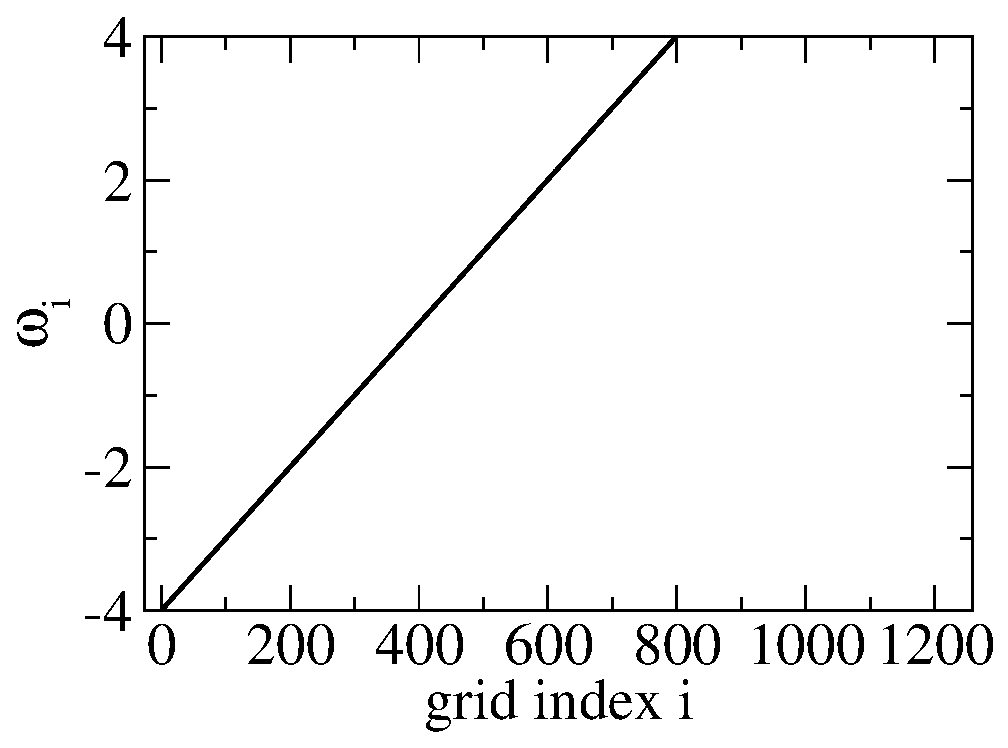
\includegraphics[width=1.0\textwidth]{pics/multigrid_00.eps}
\end{minipage}

\vspace{1cm}
After the declaration of the multigrid named \texttt{mgrid}, the member function \texttt{add\_gr\_equi} adds an equidistant grid region to the grid. The grid is created by invoking the \texttt{create} member function and it is accessed over its member variables (see table~\ref{tab:member}). 



\begin{table}[h]
	\begin{center}
		\begin{tabular}{l|l|l}\hline
		Name & Type & Description \\ \hline
		\texttt{M} & integer & Number of grid points\\\hline
		\texttt{omega} & vector & Grid (mapping $i\to\omega$ )\\\hline
		\texttt{domega} & vector & Weights of the grid\\\hline
		\texttt{omega\_min} & double & Minimum grid value (equal to \texttt{omega[0]}) \\\hline
		\texttt{omega\_max} & double & Maximum grid value (equal to \texttt{omega[M]}) \\\hline
		\texttt{inverse} & returns integer & Inverse mapping: $\omega\to i$ \\\hline
		\end{tabular}
	\end{center}
	\caption{Most important members of the multigrid}
	\label{tab:member}
\end{table}

The calculation of the above integral from $-4$ to $4$ is then done by

\begin{lstlisting}
double I=0;
for (int i=0; i<=mgrid.M; j++)
{
	I += f(mgrid.omega[i]) * mgrid.domega[i];
}
\end{lstlisting}
where the trapez rule is used to calculate the weights \texttt{domega}.

%%%%%%%%%%%%%%%%%%%%%%%%%%%%%%%%%%%%%%%%%%%%%%%%%%%%%%%%%%%%%%%%%%%%%%%%%%%%%%%%%%%%%%%%%%%%%%%%%%%%%%%%%%%%%%%%%%%
%%%%%%%%%%%%%%%%%%%%%%%%%%%%%%%%%%%%%%%%%%%%%%%%%%%%%%%%%%%%%%%%%%%%%%%%%%%%%%%%%%%%%%%%%%%%%%%%%%%%%%%%%%%%%%%%%%%
%%%%%%%%%%%%%%%%%%%%%%%%%%%%%%%%%%%%%%%%%%%%%%%%%%%%%%%%%%%%%%%%%%%%%%%%%%%%%%%%%%%%%%%%%%%%%%%%%%%%%%%%%%%%%%%%%%%
\section{Logarithmically Dense Grid Regions}\index{Grid region!logarithmic}
To resolve steps or very sharp peaks in the integrand function one needs a lot of integration grid points at specific regions. The multigrid class provides a tool to solve such problems: logarithmically dense grid regions (LGR). An LGR is determined by four variables, i.e.~the center of the grid region $\omega_0$ which corresponds for example to the position of a peak in the integrand function, the half width of the grid region $\omega_1$, the maximal resolution $d\omega_{min}$ at the center of the grid region and the minimal resolution $d\omega_{max}$ at the edges of the grid region (see figure~\ref{fig:lgr}). 
\begin{figure}[h]
	\centering
	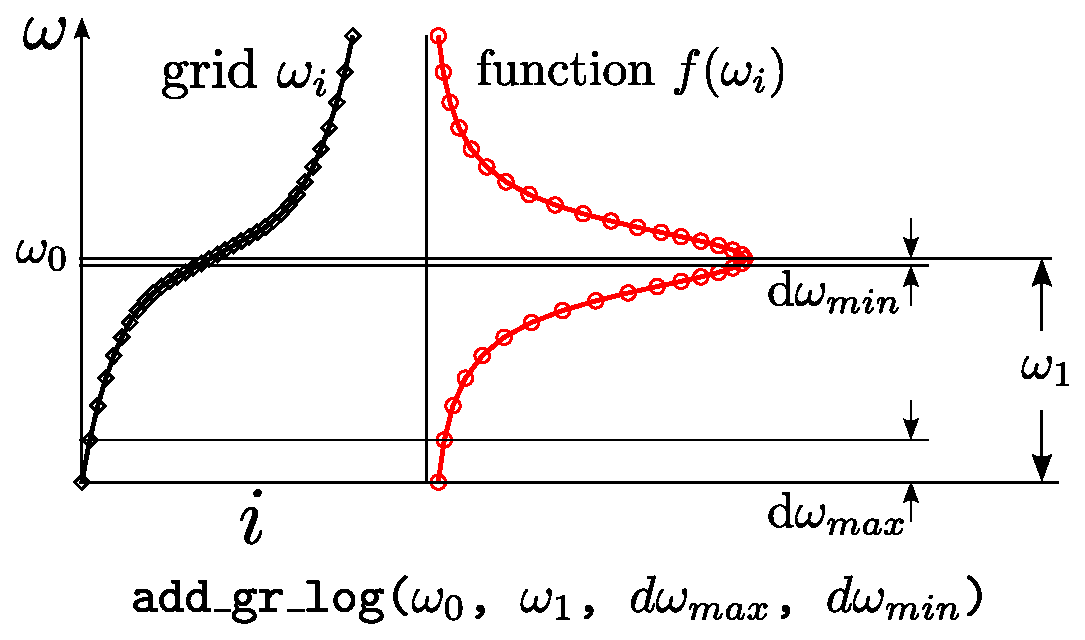
\includegraphics[width=0.6\textwidth]{pics/loggridregion.eps}
	\caption{Logarithmically dense grid region to resolve a peaked integrand function}
	\label{fig:lgr}
\end{figure}

It is created by the function \texttt{add\_gr\_log($\omega_0$, $\omega_1$, $d\omega_{max}$, $d\omega_{min}$)}. For example the following code adds a LGR on top of the equidistant grid region we used before. Note, that since the equidistant grid region was added first, it determines the outer boundaries of the whole grid (here from $-4$ to $4$). The first added grid region is therefore a special one and is called the basic grid region.
\\
\vspace{1cm}
\noindent\begin{minipage}[l]{0.6\textwidth}
\begin{lstlisting}
multigrid mgrid;
mgrid.add_gr_equi(-4, 4, 0.01);
mgrid.add_gr_log(0.3,0.5,0.001,0.01);
mgrid.create();
\end{lstlisting}
\end{minipage}
\begin{minipage}[]{0.4\textwidth}
	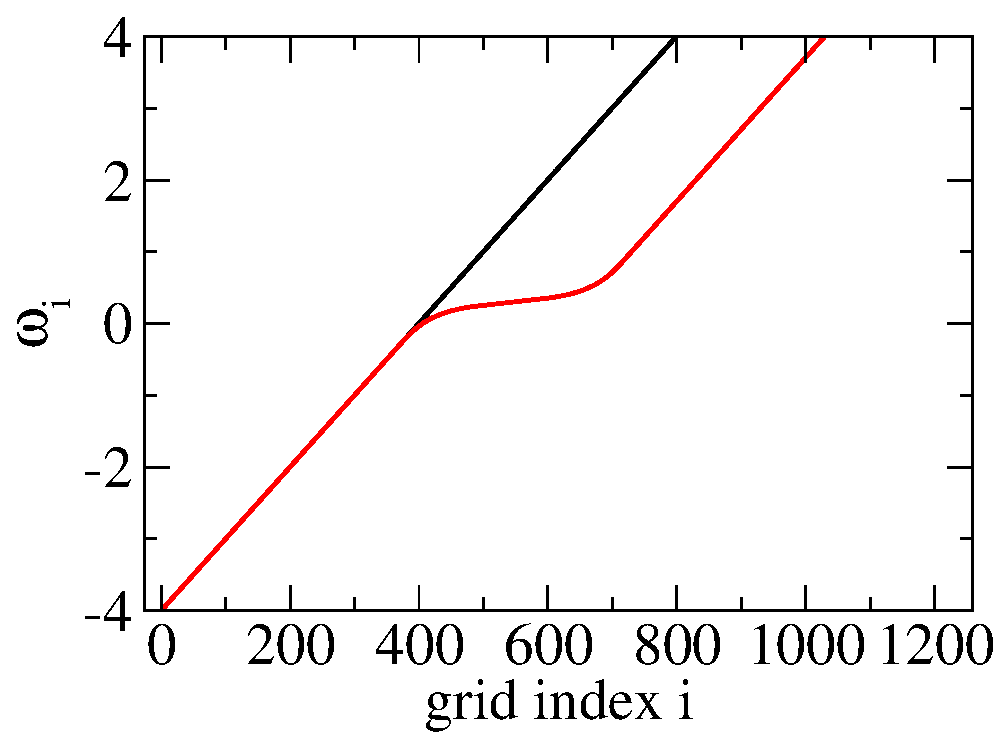
\includegraphics[width=1.0\textwidth]{pics/multigrid_01.eps}
\end{minipage}

The strength of the multigrid is that one can add now more and more grid regions on top of each other. The \texttt{create} function will take care of calculating intersection points between the grid regions by favoring the better resolved grid region. In the following example there are two intersecting LGR on top of an equidistant grid region. 
\\
\vspace{1cm}
\noindent\begin{minipage}[l]{0.6\textwidth}
\begin{lstlisting}
multigrid mgrid;
mgrid.add_gr_equi(-4, 4, 0.01);
mgrid.add_gr_log(0.3,0.5,0.001,0.01);
mgrid.add_gr_log(0.6,0.5,0.001,0.01);
mgrid.create();
\end{lstlisting}
\end{minipage}
\begin{minipage}[]{0.4\textwidth}
	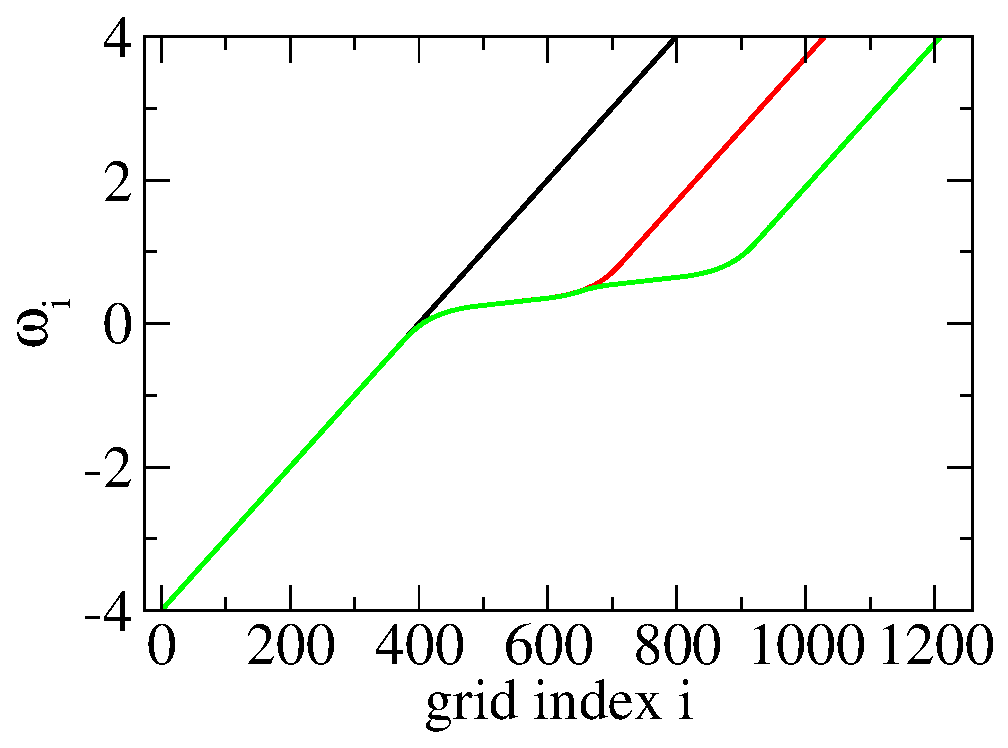
\includegraphics[width=1.0\textwidth]{pics/multigrid_02.eps}
\end{minipage}

These are only the basic features of the multigrid class. There is an algorithm which decides where to cut grid regions if there is overlap or even skip a particular grid region in special cases. The decisive element is the grid resolution exactly at the center of a given grid region. Hereby it is possible to add hundreds of grid regions on top of each other without losing the resolution at every single center point of the grid regions. In figure~\ref{fig:multiple_lgr} there is an example for the necessity for multiple LGR in the integration grid. The integrand function has several sharp peaks which have to be resolved. Each peak is resolved by a LGR.
\begin{figure}[h]
	\centering
	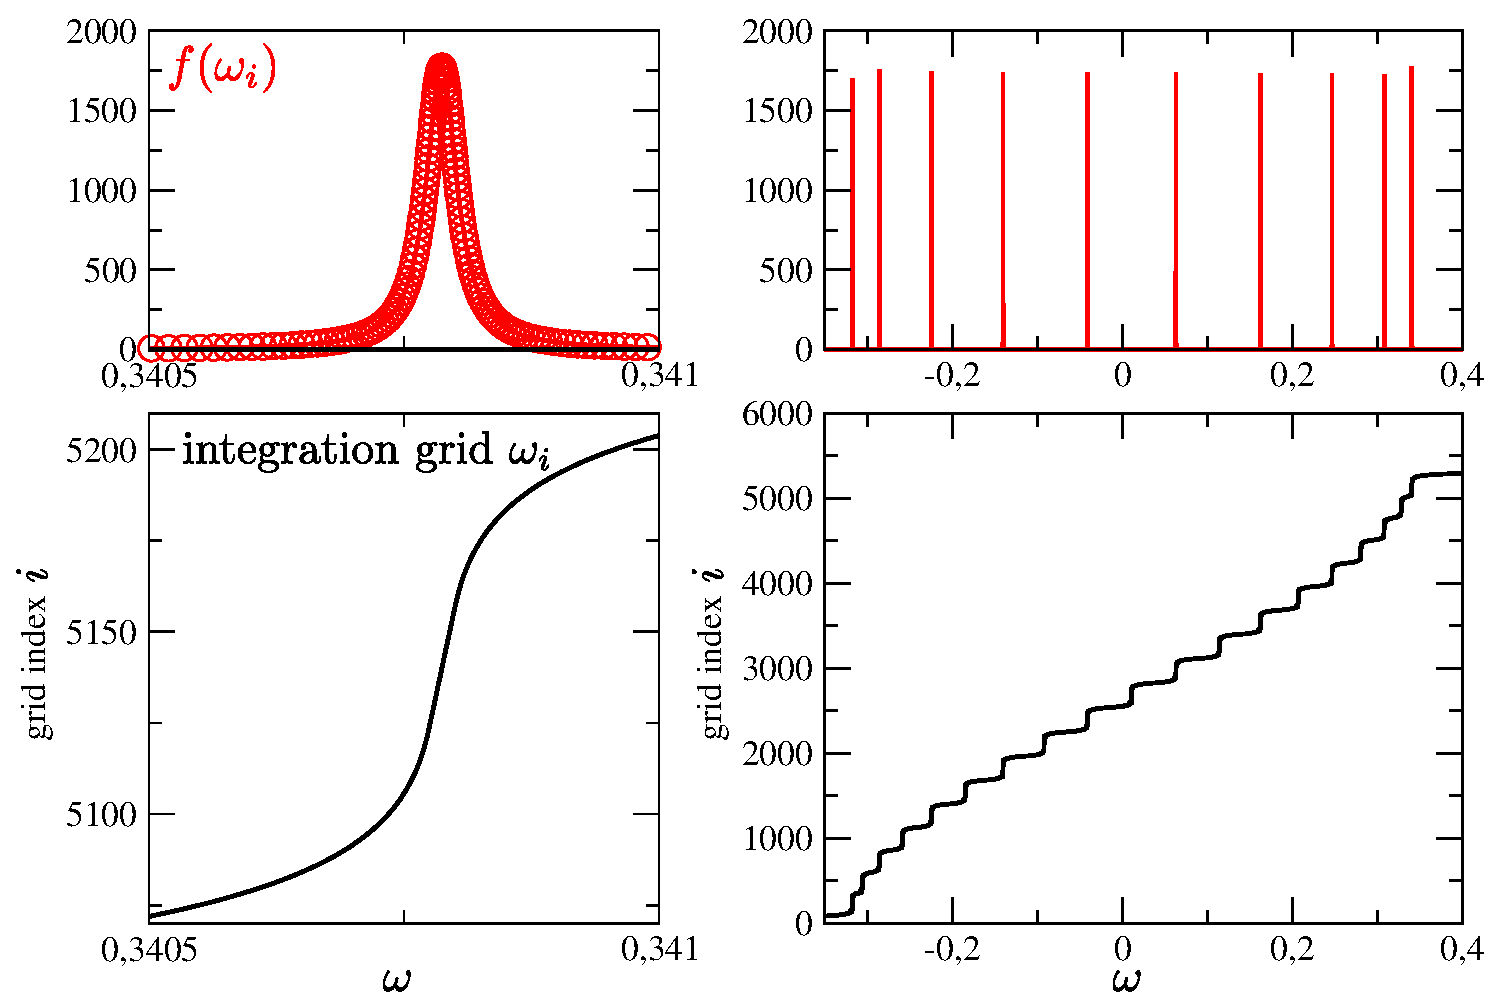
\includegraphics[width=0.9\textwidth]{pics/multiple_loggridregions.eps}
	\caption{Multigrid with various logarithmically dense grid regions to resolve a multiple peaked integrand function}
	\label{fig:multiple_lgr}
\end{figure}

\chapter{Numerical Integration}\label{chapter:numerical_integraion}
\section{Numerical Integration - Trapezoidal rule}
\index{Trapezoidal rule}
\index{Weights}
In this chapter, we will briefly review the concepts of numerical integration in one dimension. Consider an integral over some function $f(\omega)$
\begin{equation}
	I=\int_a^b d\omega f(\omega)
\end{equation}
For the numerical calculation of this integral one has to discretize the interval of integration $[a,b]$:
\[
	\omega(i) \quad;\quad i\in\{0,\dots,M\}\quad\text{and}\quad \omega(0)=a,\quad \omega(M)=b.
\]
Where the strictly increasing mapping $\omega: \mathbbm{N} \to \mathbbm{R}: i \mapsto \omega(i)$ is called a grid. The numerical approximation for the integral now reads
\begin{equation} 
	I=\sum_{i=0}^M d\omega(i) f(\omega(i))
\end{equation}
where the $d\omega(i)$ are the so-called weights. There are various methods to calculate the weights out of the grid itself. We will restrict ourselves to the trapezoidal rule which approximates the integrand function by linear regions connecting the sample points (see figure~\ref{fig:trapezoidal_rule}).
\begin{figure}[ht]
	\centering
	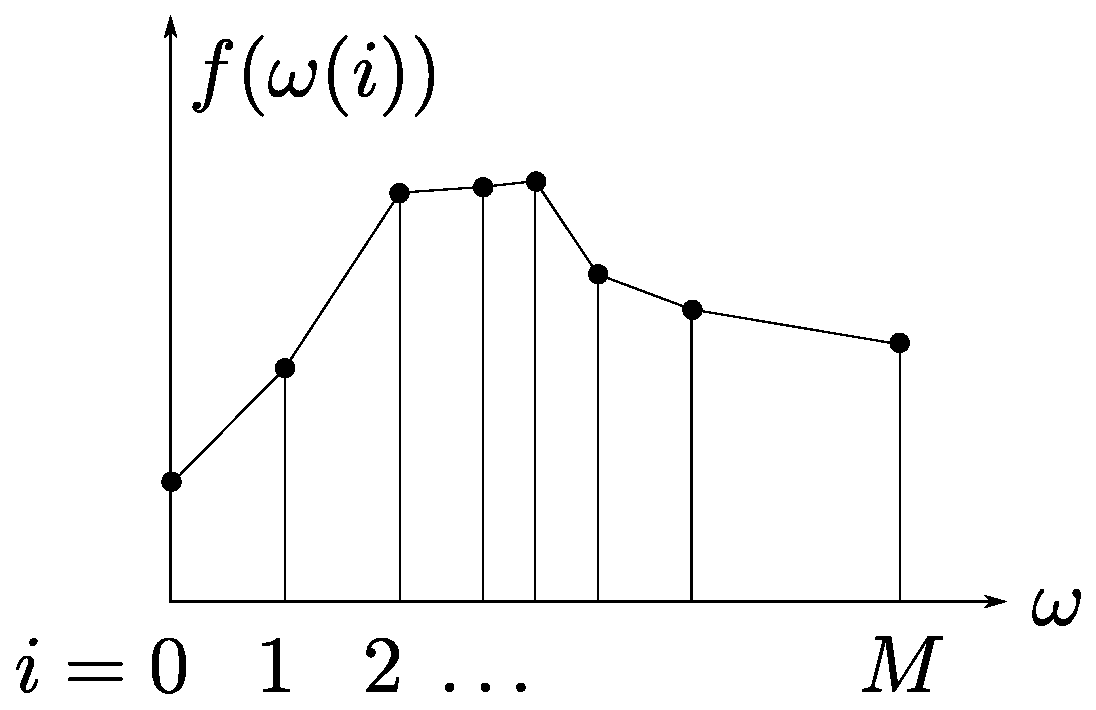
\includegraphics[width=0.3\textwidth]{pics/trapez.eps}
	\caption{Trapezoidal rule for a non-equidistant grid.}
	\label{fig:trapezoidal_rule}
\end{figure}

The numerical approximation for the integral is then
\begin{align*}
	I&=\sum_{i=0}^{M-1} \frac{f(\omega(i+1)) + f(\omega(i))}{2} (\omega(i+1)-\omega(i)) \\
	&=f(a)\biggl( \underbrace{\frac{\omega(1)-\omega(0)}{2}}_{d\omega(0)}\biggr) + f(b) \biggl( \underbrace{\frac{\omega(N)-\omega(N-1)}{2}}_{d\omega(N)}\biggr) + \sum_{i=1}^{M-1} f(\omega(i)) \biggl( \underbrace{\frac{\omega(i+1)-\omega(i-1)}{2}}_{d\omega(i)}\biggr)\\
	&=\sum_{i=0}^{M} d\omega(i)\,f(\omega(i)).
\end{align*}
Therefore the weights are given by
\[
	d\omega(i)=\begin{cases}
		\frac{\omega(1)-\omega(0)}{2} \quad &i=0\\
		\frac{\omega(i+1)-\omega(i-1)}{2} \quad &i\in \{1,\dots,M-1\}  \\
		\frac{\omega(N)-\omega(N-1)}{2} \quad &i=\,.
	\end{cases}
\]

\section{Interpolation - Inverse mapping}\index{Interpolation}
\index{Inverse mapping}
In order to calculate a function $f$ which is known on a given grid $\omega(i)$, on another grid $\epsilon(i)$ one needs to interpolate. We restrict ourselves to linear interpolation and we further assume, that the inverse mapping of the first grid
\[
	i(\omega):\;\mathbbm{R}\to\mathbbm{N}:\quad \omega \mapsto i\quad\quad;\;\omega\in[\omega(0), \omega(M)]
\]
is known.

The interpolation is then done in the following way. For each point of the new grid $\epsilon(j)\equiv \epsilon_j$ one calculates the inverse of the old grid $I=i(\epsilon_j)$. The corresponding old grid point $\omega(I)\equiv \omega_I$ is then the nearest grid point to the interpolation point $\epsilon_j$ (Figure~\ref{fig:interpolation}). 
\begin{figure}[ht]
	\centering
	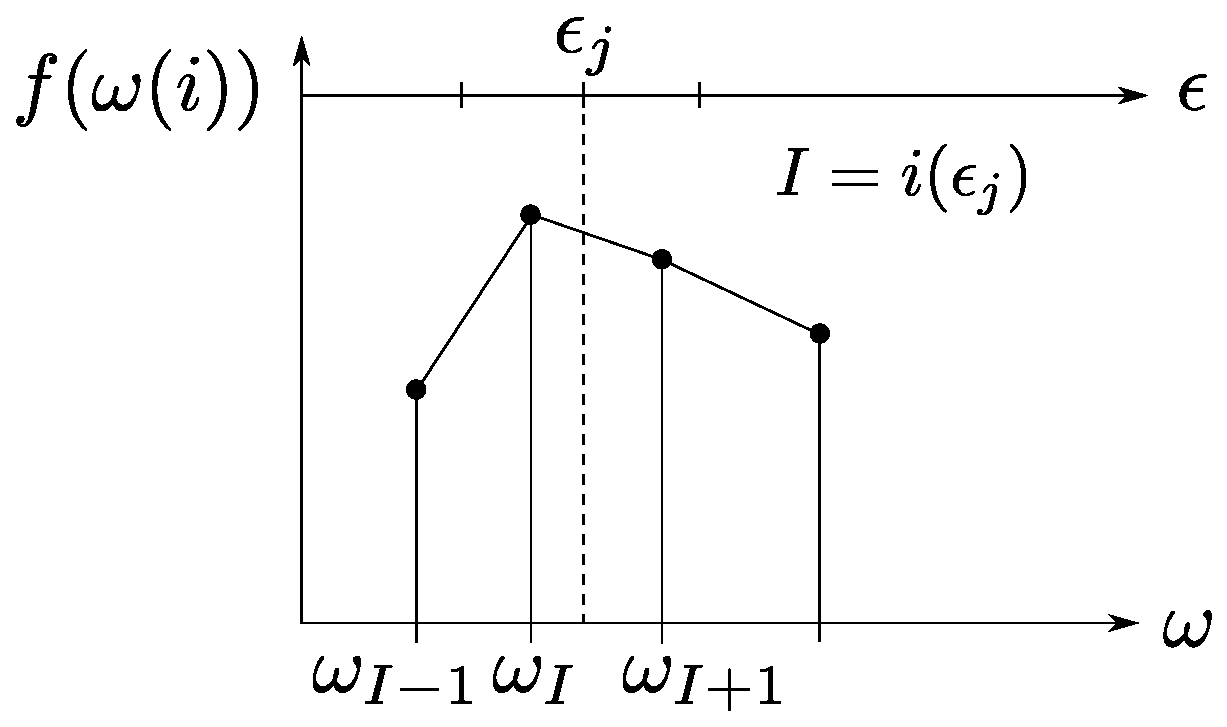
\includegraphics[width=0.4\textwidth]{pics/interpolation.eps}
	\caption{Linear interpolation of $f(\{\omega_i\})$ on a new grid $\{ \epsilon_j \}$}
	\label{fig:interpolation}
\end{figure}

The value of the function on a point $\epsilon_j$ of the new grid $f(\epsilon_j)$ is then obtained by linear interpolation between the old grid point $\omega_I$ and its nearest neighbor (right neighbor for $\omega_I\leq\epsilon_j$, left neighbor for $\omega_I>\epsilon_j$).
\[
	f(\epsilon_j)=\begin{cases}
		f(\omega_I)+\frac{f(\omega_{I+1})-f(\omega_{I})}{\omega_{I+1}-\omega_{I}} (\epsilon_j-\omega_I) \quad \text{for } \omega_I<\epsilon_j \\
		f(\omega_I)+\frac{f(\omega_{I-1})-f(\omega_{I})}{\omega_{I-1}-\omega_{I}} (\epsilon_j-\omega_I) \quad \text{for } \omega_I>\epsilon_j 
	\end{cases}
\]







\chapter{Simple grids} \label{chapter:simple_grids}
In the following we will introduce all kinds of available grids together with their numerical structure. These grids will be the building blocks of the multigrid.
\section{The base class: grid}\index{Grid!class}
As it was shown in chapter \ref{chapter:numerical_integraion} all one needs for numerical integration is the integration grid itself and the corresponding weights. All of this is comprised in the class \texttt{grid} whose members are listed in table \ref{tab:member}. The grid class is defined in the \texttt{grid.h} file as follows

\begin{lstlisting}
class grid
{
        public:
        int M;
        double omega_min;
        double omega_max;
        vector <double> omega;
        vector <double> domega;
        virtual unsigned int inverse (double omega)=0;
};
\end{lstlisting}
The grid itself and its weights are \texttt{vectors} \cite{stl}. The inverse mapping is virtual, and so is the grid class itself. Only the classes which are derived from the grid class are non-virtual. If one is not familiar with the concept of inheritance one can think of it in the following way: Since all integration grids should possess the above attributes (table \ref{tab:member}), it is reasonable to define a skeleton for an integration grid. This is the virtual grid class. It is not possible to create an instance of the grid class, but its possible to give it as an argument in a function. For example:
\begin{lstlisting}
void saveGrid(grid & mgrid, string filename)
{
        ofstream out;
        out.open(filename.c_str());
        for (int j=0; j!=mgrid.M+1; j++)
        {
                out << j << "\t" << mgrid.omega[j] << endl;
        }
        out.close();
}
\end{lstlisting}
This function can then take any kind of grid class (as long as it is derived from the basic grid class) as an argument (for an example, see section \ref{sec:using_the_grid_classes}). This is the whole purpose of using a virtual base grid class. In the following we will introduce all kinds of available grids.

\section{Equidistant grid: equigrid}\label{sec:equigrid}
\index{Grid!equidistant}
\index{equigrid}

The simplest grid class is the equidistant grid class. It is called \texttt{equigrid} and the grid is defined in the following way
\[
	\omega(i) = \omega_{min} + d\omega \cdot i\,,
\]
with $i\in {0,\dots,M}$ and $\omega(M)=\omega_{max}$. Beside the grid class attributes (table \ref{tab:member}), the equigrid has only one additional variable: the grid resolution $d\omega$. The inverse of $\omega(i)$ is given by
\[
	i(\omega)=\frac{\omega-\omega_{min}}{d\omega}
\]
The grid point density reads
\begin{equation}\label{eqn:equigrid_grid_point_density}
 \frac{di}{d\omega} (\omega) = \frac{1}{d\omega}
\end{equation}
The class is defined in the files \texttt{grid.h} and \texttt{grid.cpp}. Its defining member variables are listed in table \ref{tab:equigrid_defining_members}.
\begin{table}[h]
	\begin{center}
		\begin{tabular}{llp{3cm}l}
		Name            & Member                     & Constructor & Description           \\ 
		                &                            & Argument    &                       \\
		\hline
		$M$             & \texttt{int M}             & \nth{1}     & Number of grid points \\
		$\omega_{min}$  & \texttt{double omega\_min} & \nth{2}     & Lower boundary        \\
		$\omega_{max}$  & \texttt{double omega\_max} & \nth{3}     & Upper boundary        \\
		\end{tabular}
	\end{center}
	\caption{Defining properties of the \texttt{equigrid} class}
	\label{tab:equigrid_defining_members}
\end{table}
These are also the arguments of the equigrid constructor which is used for creating an instance of an equigrid:
\begin{lstlisting}
equigrid egrid(M, omega_min, omega_max);
\end{lstlisting}


\section{Tangential grid: tangrid}\label{sec:tangrid}
\index{Grid!tangential}
\index{tangrid}

The tangential grid is called \texttt{tangrid}. Beside the grid class attributes (table \ref{tab:member}), it has a cluster point at $\omega_c$: \\

\begin{center}
	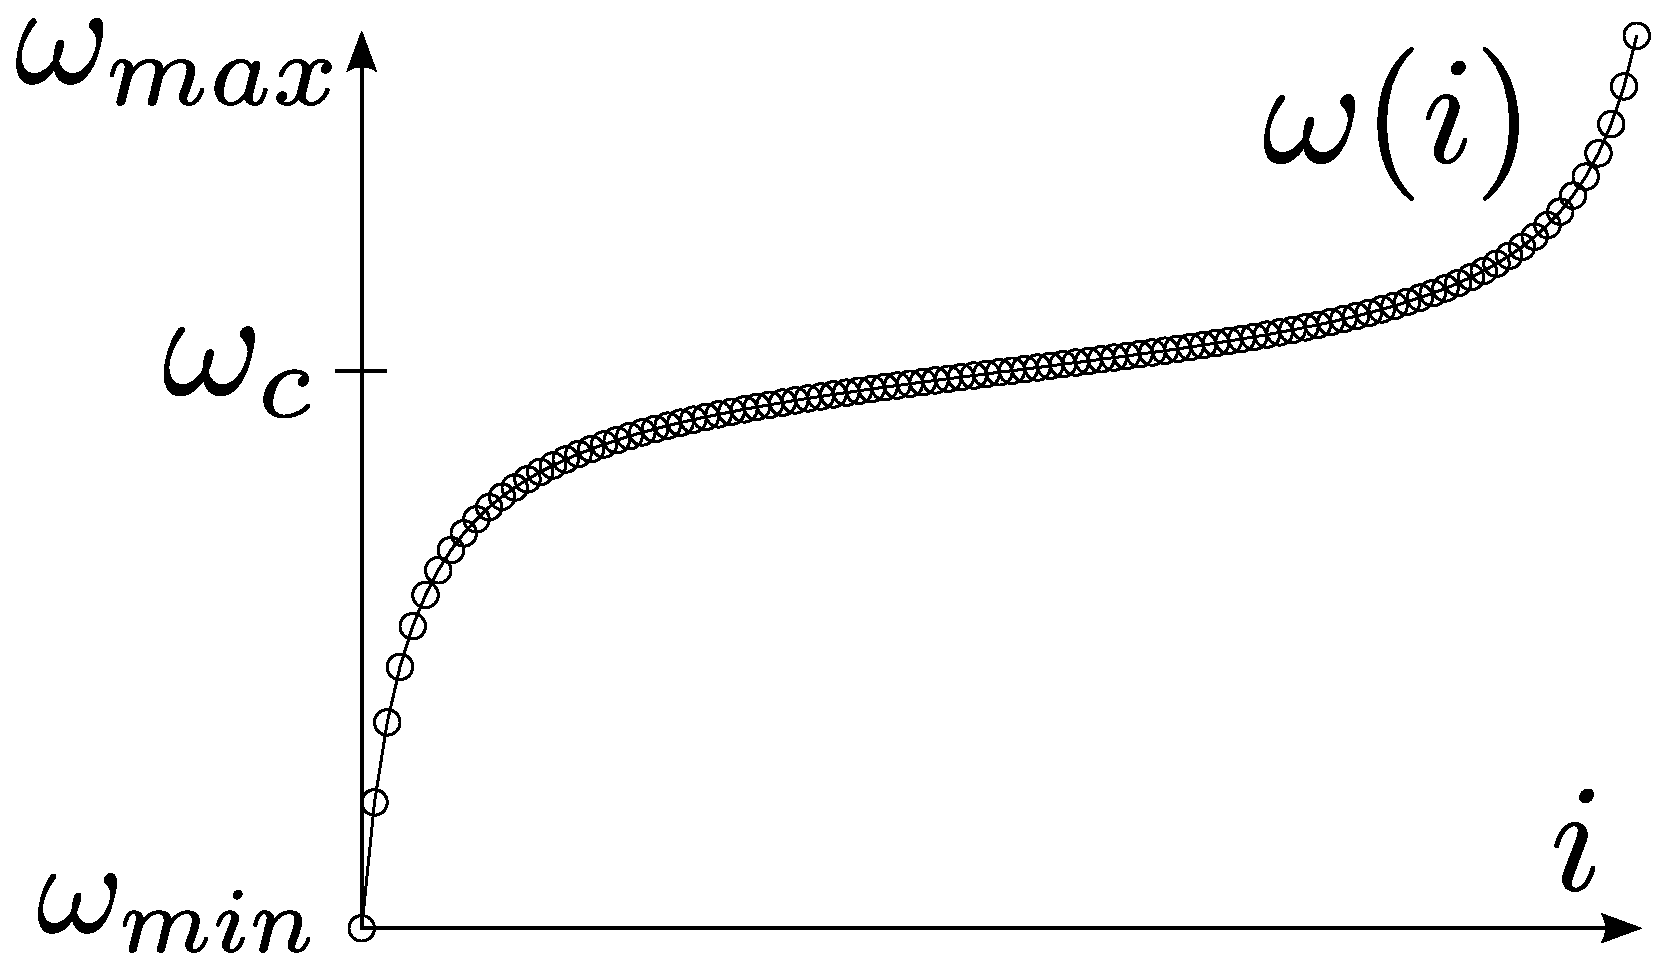
\includegraphics[width=0.3\textwidth]{pics/tangrid.eps}
\end{center}

\noindent The ``sharpness`` of this curve is controlled by the parameter $c$ and the grid is defined by
\[
	\omega(i)= c \tan (u_1+\Delta u \cdot i) + \omega_c
\]
where $i\in \{0,\dots,M\}$, and the parameters $u_1$ and $\Delta u$ are calculated such, that boundary conditions $\omega(0)=\omega_{min}$ and $\omega(M)=\omega_{max}$ are fulfilled. Hence:
\begin{align*}
	u_1&=\arctan\left(\frac{\omega_{min}-\omega_c}{c}\right)\\
	u_2&=\arctan\left(\frac{\omega_{max}-\omega_c}{c}\right)\\
	\Delta u&=\frac{u_2-u_1}{M}
\end{align*}
The inverse of the grid is given by
\[
	i(\omega)=\frac{1}{\Delta u}\left(\arctan\left(\frac{\omega-\omega_c}{c}\right)-u_1\right)
\]
and the point density reads
\begin{equation}\label{eqn:tangrid_grid_point_density}
 \frac{di}{d\omega} (\omega) = \frac{1}{c \Delta u\left(1+\left(\frac{\omega-\omega_c}{c}\right)^2\right)}\,.
\end{equation}

The class is defined in the files \texttt{grid.h} and \texttt{grid.cpp}. Its defining member variables are listed in table \ref{tab:tangrid_defining_members}.
\begin{table}[h]
	\begin{center}
		\begin{tabular}{llll}
		Name            & Member                     & Constructor & Description           \\ 
		                &                            & Argument    &                       \\ 
		\hline
		$M$             & \texttt{int M}             & \nth{1}     & Number of grid points \\
		$\omega_{min}$  & \texttt{double omega\_min} & \nth{2}     & Lower boundary        \\
		$\omega_{max}$  & \texttt{double omega\_max} & \nth{3}     & Upper boundary        \\
		$\omega_{c}$    & \texttt{double omega\_c}   & \nth{4}     & Center point          \\
		$c$             & \texttt{double c}          & \nth{5}     & Controls sharpness   \\
		\end{tabular}
	\end{center}
	\caption{Defining properties of the \texttt{tangrid} class}
	\label{tab:tangrid_defining_members}
\end{table}
These are also the arguments of the tangrid constructor which is used for creating an instance of a tangrid:
\begin{lstlisting}
tangrid tgrid(M, omega_min, omega_max, omega_c, c);
\end{lstlisting}

\section{Logarithmic grid: loggrid}\label{sec:loggrid}
\index{Grid!logarithmic}
\index{loggrid}
To resolve very sharp peaks in the integrand function the logarithmic grid is the right tool. It is named \texttt{loggrid} and it is constructed in the following way. There are three grid regions: one below (I), one around (II) and one above (III) the center point $\omega_k$, which is the point with the highest grid point density.\\

\begin{center}
	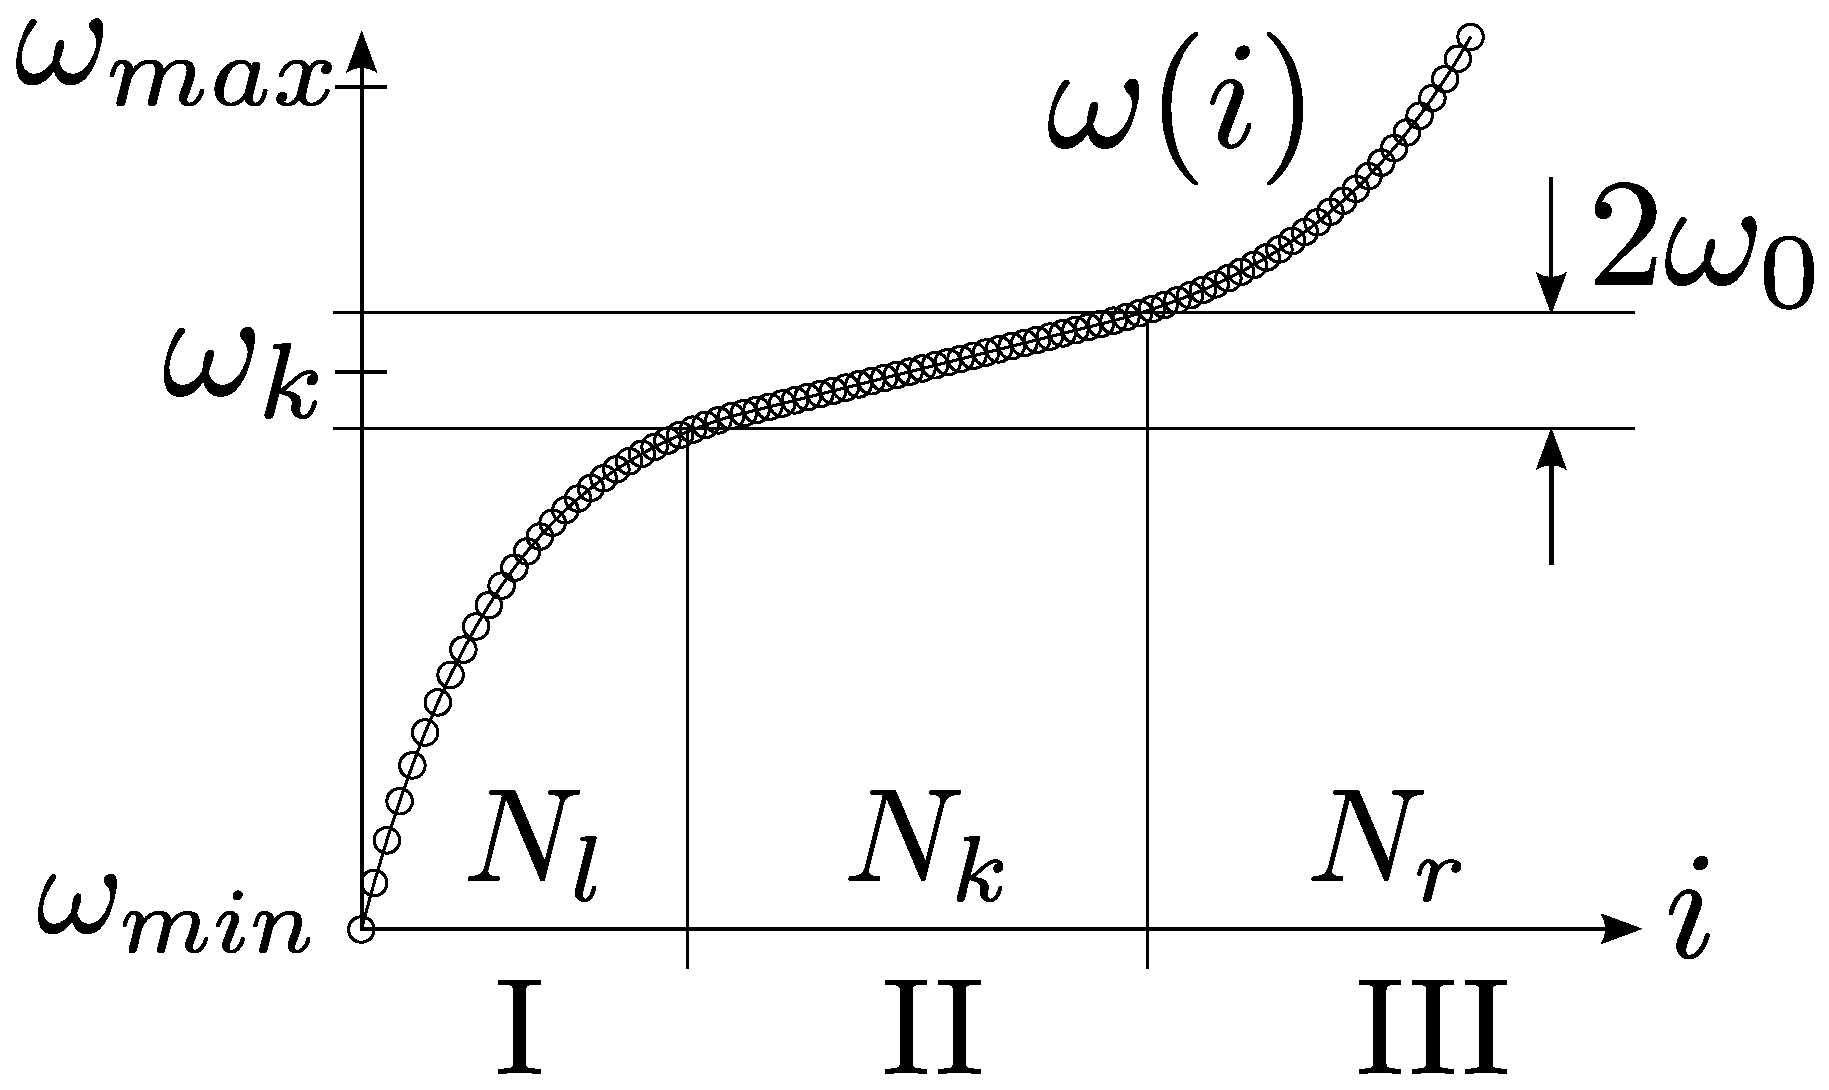
\includegraphics[width=0.4\textwidth]{pics/loggrid.eps}
\end{center}

Region I and III are exponential and region II is linear. The half width of the linear region $\omega_0$ also controls the ''sharpness`` of the exponential grid regions. The number of grid points in region I, $N_l$ and in region III, $N_r+1$ can be chosen different from each other. Both will also influence the ''sharpness'' of the exponential grid regions. The resolution of the linear grid region $d\omega_k$ is the same as the maximal resolution in the exponential grid regions and it determines the number of grid points in region II, $N_k$ (see Appendix \ref{sec:app_loggrid_max_resolution}). The grid is defined as
\begin{equation}\label{eqn:loggrid_definition}
	\omega(i)=\begin{cases}
		-\exp(-c_1(i-i_1)) + \omega_k 		\quad & i\in\{0,\dots,N_l-1\} \\ 
		\omega_k-\omega_0+d\omega_k(i-N_l-1)	\quad & i\in\{N_l,\dots,N_l+N_k-1\} \\ 
		\exp(c_2(i-i_2-N_l-N_k)) + \omega_k 	\quad & i\in\{N_l+N_k,\dots,N_l+N_k+N_r\}
	\end{cases}
\end{equation}
The four boundary conditions
\begin{align}\label{eqn:loggrid_boundary_conditions}
	\omega(0)&=\omega_{min} \quad &\omega(N_l-1)&=\omega_k-\omega_0 \notag \\
	\omega(N_l+N_k)&=\omega_k+\omega_0 \quad &\omega(N_l+N_k+N_r)&=\omega_{max}
\end{align}
determine the four parameters $i_1$, $i_2$, $c_1$ and $c_2$ (see Appendix \ref{sec:app_loggrid_boundary}). The inverse is given by
\[
	i(\omega)=\begin{cases}
		\frac{\log(\omega_k-\omega)}{-c_1} + i_1 \quad &\text{for } \omega\in[\omega_{min},\omega_k-\omega_0] \\
		\frac{\omega-\omega_k+\omega_0}{d\omega_k} + N_l -1\quad &\text{for } \omega\in(\omega_k-\omega_0,\omega_k+\omega_0) \\
		\frac{\log(\omega-\omega_k)}{c_2} + i_2 + N_l + N_k \quad &\text{for } \omega\in[\omega_k+\omega_0, \omega_{max}]
	\end{cases}
\]
and the grid point density reads
\begin{equation}\label{eqn:loggrid_grid_point_density}
	\frac{di(\omega)}{d\omega}=\begin{cases}
		\frac{1}{c_1(\omega_k-\omega)} \quad &\text{for } \omega\in[\omega_{min},\omega_k-\omega_0) \\
		\frac{1}{d\omega_k} \quad &\text{for } \omega\in[\omega_k-\omega_0,\omega_k+\omega_0) \\
		\frac{1}{c_2(\omega-\omega_k)}  \quad &\text{for } \omega\in[\omega_k+\omega_0, \omega_{max}]
	\end{cases}
\end{equation}

The class is defined in the files \texttt{grid.h} and \texttt{grid.cpp}. Its defining member variables are listed in table \ref{tab:loggrid_defining_members}.
\begin{table}[h]
	\begin{center}
		\begin{tabular}{llll}
		Name            & Member                     & Constructor          & Description                         \\ 
		                &                            & Argument             &                                     \\ 
		\hline
		$N_l$           & \texttt{int N\_l}          & \nth{1}              & Number of grid points in region I   \\
		$N_r$           & \texttt{int N\_r}          & \nth{2}              & Number of grid points in region III \\
		$\omega_{min}$  & \texttt{double omega\_min} & \nth{3}              & Lower boundary                      \\
		$\omega_{max}$  & \texttt{double omega\_max} & \nth{4}              & Upper boundary                      \\
		$\omega_{k}$    & \texttt{double omega\_k}   & \nth{5}              & Center point                        \\
		$\omega_{0}$    & \texttt{double omega\_0}   & \nth{6}              & Half width of the region II         \\
		\end{tabular}
	\end{center}
	\caption{Defining properties of the \texttt{loggrid} class}
	\label{tab:loggrid_defining_members}
\end{table}
These are also the arguments of the loggrid constructor which is used for creating an instance of a loggrid:
\begin{lstlisting}
loggrid loggrid(N_l, N_r, omega_min, omega_max, omega_k, omega_0);
\end{lstlisting}

\section{Using the grid classes}\label{sec:using_the_grid_classes}
\index{equigrid}
\index{tangrid}
\index{loggrid}

All of the above grids are derived from the base class \texttt{grid}. Therefore it is possible to write a function which performs the numerical integration without specifying the type of grid one wants to use
\begin{lstlisting}
double integrate(double (&f)(double), grid & g)
{
	double I=0
	for (int i=0; i<=mgrid.M; i++)
	{
		I+= f(mgrid.omega[i]) * domega[i];
	}
	return I;
} 
\end{lstlisting}
which can then be used for example with an equigrid and a Gauss function
\begin{lstlisting}
double gauss(double x)
{
	return exp(-x*x);
}
int main()
{
        equigrid agrid(100, -4, 4);
        //tangrid agrid(100, -4, 4, 1, 0.5);
        //loggrid agrid(30, 30, -4, 4, 1, 0.4);
        double I=integrate(gauss, agrid);
}
\end{lstlisting}
But one can also change the comments in the code in such a way, that a tangrid or a loggrid is used for the integration of a Gauss function.




\chapter{Multigrid} \label{chapter:multigrid_usage}
In this chapter we will introduce all the knowledge which is required for the usage of the multigrid. In order to understand the selection and cutting procedure which is the very heart of the multigrid class we refer to chapter \ref{chapter:multigrid_selection_and_cutting}.
\index{Multigrid}

\section{Overview}
A multigrid consists of a single basic grid region which defines the outer boundaries of the multigrid and multiple grid regions. Each of these grid regions can be equidistant, tangential or logarithmic. If the grid regions overlap with each other, they will be cut in such a way, that the grid resolution remains constant while crossing over the cutting point. It could also happen that a particular grid region is forced out by another grid region because the purpose of the former one is already served by the latter one. How this is done in detail will be part of chapter \ref{chapter:multigrid_selection_and_cutting}.

A multigrid is created in the following way (see listing \ref{lst:create_multigrid_sketch}). First it has to be initialized. Afterwards one can add, replace and remove multiple grid regions. This will be explained in detail in section \ref{sec:grid_regions}. Finally the member function \texttt{create} is invoked. Hereby the cutting and selection procedure will be performed and the multigrid will be created. 
\begin{lstlisting}[caption={Creating a multigrid},	label={lst:create_multigrid_sketch}]
multigrid mgrid;
... 
... //add, replace and remove grid regions
...
mgrid.create()
\end{lstlisting}
The multigrid is also derived from the grid class and can therefore be used exactly in the same way as the other grids (see section \ref{sec:using_the_grid_classes})

\section{Grid regions}\label{sec:grid_regions}
\index{Grid region}
In this chapter we will introduce the notion of a grid region. We will assume, that the purpose of a grid region is to resolve some feature of the integrand function which is located at a single point. This will be the center point of the grid region, $\omega_c$. Together with the left and right boundaries $\omega_l$ and $\omega_r$, the type of grid region (equidistant, tangential or logarithmic) and the grid region parameters (e.g. $\omega_k$ and $\omega_0$ for the loggrid) these are the defining properties of a grid region. The grid region is implemented as a class named \texttt{gridRegion} and is defined in the file \texttt{multigrid.h}. Its defining member variables are shown in table \ref{tab:grid_region_defining_members}.
\begin{table}[h]
	\begin{center}
		\begin{tabular}{ll}
		Name & Description \\ 
		\hline
		$\omega_c$  & Center point \\
		$\omega_l$  & Lower boundary \\
		$\omega_r$  & Upper boundary \\
		\texttt{type}  & Type of grid region \\
		\texttt{id}  & Name of the grid region (optional) \\
		 $\dots$ & Grid region parameters (e.g. $\omega_k$ and $\omega_0$ for the loggrid) \\
		\end{tabular}
	\end{center}
	\caption{Defining properties of the grid region}
	\label{tab:grid_region_defining_members}
\end{table}

It is obvious, that a possible cutting point can not be arbitrarily narrow to the center point $\omega_c$. For example in the loggrid case, for numerical reasons at least three points of the exponential grid regions must survive in order to have a starting, an intermediate and an endpoint of this region. Also the corresponding weights should not be smaller than the machine precision. Therefore one introduces a buffer region around $\omega_c$ which is defined by its upper and lower boundaries $\omega_+$ and $\omega_-$. In section \ref{sec:cutting_procedure} we will see, that in order to calculate the cutting point according to the grid point density (grid resolution) the maximal grid resolution on both sides of the center point, $d\omega_l$ and $d\omega_r$, is necessary. Hereby we assume that the grid point density is monotonically increasing from the boundaries towards the center of the grid region. (This is true for all three kinds of grids from chapter \ref{chapter:simple_grids}). Table \ref{tab:grid_region_derived_members} shows the relevant derived properties of the grid region class, i.e. they are calculated directly out of the defining properties.
\begin{table}[h]
	\begin{center}
		\begin{tabular}{ll}
		Name & Description \\ 
		\hline
		$\omega_+$  & Upper boundary of the buffer region around $\omega_c$ \\
		$\omega_-$  & Lower boundary of the buffer region around $\omega_c$ \\
		$d\omega_l$  & Maximal resolution left to $\omega_c$ \\
		$d\omega_r$  & Maximal resolution right to $\omega_c$ \\
		\end{tabular}
	\end{center}
	\caption{Relevant derived properties of the grid region}
	\label{tab:grid_region_derived_members}
\end{table}

Note that there are actually more member variables. But since they will never appear to the user we will not discuss them here. In the following we will introduce the different kinds of grid regions. There are equidistant, tangential and logarithmic grid regions. Naturally, the boundaries of a particular grid region $\omega_l$ and $\omega_r$ will correspond to the boundary $\omega_{min}$ and $\omega_{max}$ of the simple grids from chapter \ref{chapter:simple_grids}. In table \ref{tab:grid_region_types} the mapping from the grid class member variables to the grid region member variables is shown. As mentioned earlier, the boundaries of the buffer region around the center point are chosen such, that there will be 3 points left. In the case of the logarithmic grid region, the buffer region always includes the linear region II of the loggrid. Note, that the center point of the equidistant grid region can be chosen arbitrarily.
\begin{table}[h]
	\begin{center}
		\begin{tabular}{llll}
		Grid region & equidistant & tangential & logarithmic  \\ 
		variable    &             &            &              \\
		\hline 
		$\omega_c$    & -               & $\omega_c$     & $\omega_k$     \\
		$\omega_l$    & $\omega_{min}$  & $\omega_{min}$ & $\omega_{min}$ \\
		$\omega_r$    & $\omega_{max}$  & $\omega_{max}$ & $\omega_{max}$ \\
		\texttt{type} & \texttt{'equi'} & \texttt{'tan'} & \texttt{'log'} \\
		$\omega_+$         & $\omega_c+3d\omega$ & $\omega_c+3c\Delta u$ & $\omega(i=N_l+N_k+3)$ \\
		$\omega_-$         & $\omega_c-3d\omega$ & $\omega_c-3c\Delta u$ & $\omega(i=N_l-3)$  \\
		$d\omega_l$  & $d\omega$ & $c\Delta u$ & see Appendix \ref{sec:app_loggrid_max_resolution} \\
		$d\omega_r$  & $d\omega$ & $c\Delta u$ & see Appendix \ref{sec:app_loggrid_max_resolution} \\
		\end{tabular}
	\end{center}
	\caption{Relation of grid class and grid region member variables}
	\label{tab:grid_region_types}
\end{table}

\subsection{Adding grid regions}\label{subsec:grid_region_adding}
\index{Grid region!equidistant}
\index{Grid region!tangential}
\index{Grid region!logarithmic}
\index{Grid region!add}
In this section we introduce the syntax for adding grid regions to the multigrid. (See section \ref{subsec:grid_region_examples} for examples).
An equidistant grid region consists of an instance of an equigrid (see \ref{sec:equigrid}). It is added to the multigrid by the member function 
\begin{lstlisting}
void add_gr_equi
\end{lstlisting}
Its arguments are shown in table \ref{tab:add_gr_equi}.

\begin{table}[h]
	\begin{center}
		\begin{tabular}{lll}		
		Argument  & Type & Description \\ \hline
		\nth{1}   & \texttt{int}    & Number of grid points ($M$) \\ 
		\nth{2}   & \texttt{double} & Lower boundary ($\omega_l$) \\ 
		\nth{3}   & \texttt{double} & Upper boundary ($\omega_r$) \\ 
		\nth{4}   & \texttt{double} & Center point ($\omega_c$) \\ 
		(\nth{5}) & \texttt{string} & Name of the grid region (\texttt{id})(optional)\\ 
		\end{tabular}
	\end{center}
	\caption{Arguments of the member function \texttt{add\_gr\_equi}}
	\label{tab:add_gr_equi}
\end{table}

A tangential grid region consists of an instance of a tangrid (see \ref{sec:tangrid}). It is added to the multigrid by the member function 
\begin{lstlisting}
void add_gr_tan
\end{lstlisting}
Its arguments are shown in table \ref{tab:add_gr_tan}.

\begin{table}[h]
	\begin{center}
		\begin{tabular}{lll}		
		Argument  & Type & Description \\ \hline
		\nth{1}   & \texttt{int}    & Number of grid points ($M$) \\ 
		\nth{2}   & \texttt{double} & Lower boundary ($\omega_l$) \\ 
		\nth{3}   & \texttt{double} & Upper boundary ($\omega_r$) \\ 
		\nth{4}   & \texttt{double} & Center point ($\omega_c$) \\ 
		\nth{5}   & \texttt{double} & Controls sharpness ($c$) \\ 
		(\nth{6}) & \texttt{string} & Name of the grid region (\texttt{id})(optional)\\ 
		\end{tabular}
	\end{center}
	\caption{Arguments of the member function \texttt{add\_gr\_tan}}
	\label{tab:add_gr_tan}
\end{table}

A logarithmic grid region consists of an instance of a loggrid (see \ref{sec:loggrid}). It is added to the multigrid by the member function 
\begin{lstlisting}
void add_gr_log
\end{lstlisting}
Its arguments are shown in table \ref{tab:add_gr_log}.

\begin{table}[h]
	\begin{center}
		\begin{tabular}{lll}		
		Argument  & Type & Description \\ \hline
		\nth{1}   & \texttt{int}    & Number of grid points in region I ($N_l$) \\ 
		\nth{2}   & \texttt{int}    & Number of grid points in region III ($N_r$) \\ 
		\nth{3}   & \texttt{double} & Lower boundary ($\omega_l$) \\ 
		\nth{4}   & \texttt{double} & Upper boundary ($\omega_r$) \\ 
		\nth{5}   & \texttt{double} & Center point ($\omega_k$) \\ 
		\nth{6}   & \texttt{double} & Half width of region II ($\omega_0$) \\ 
		(\nth{7}) & \texttt{string} & Name of the grid region (\texttt{id})(optional)\\ 
		\end{tabular}
	\end{center}
	\caption{Arguments of the member function \texttt{add\_gr\_log}}
	\label{tab:add_gr_log}
\end{table}

\subsection{Replacing and removing grid regions}\label{subsec:grid_region_replace_remove}
\index{Grid region!equidistant}
\index{Grid region!tangential}
\index{Grid region!logarithmic}
\index{Grid region!replace}
\index{Grid region!remove}
After adding a lot of grid regions to the multigrid there may be a situation were one wants to change only a single grid region out of many. This can be achieved by replacing that particular grid region by another one with different parameters.
We have seen, that if a grid region is added to the multigrid, it is optional to give a name to this grid region. In contrast to that, you can only replace or remove grid regions which have a name. One can check if a grid region with the name \texttt{id} exists, by calling the member function
\begin{lstlisting}
bool gr_exists(string id)
\end{lstlisting}
If this is the case one can remove it by
\begin{lstlisting}
void rem_gr(string id)
\end{lstlisting}
In order to replace a grid region by one with the same name but different attributes one calls one of the replace member functions
\begin{lstlisting}
void replace_gr_equi(...)
void replace_gr_tan(...)
void replace_gr_log(...)
\end{lstlisting}
where the arguments are exactly the same as for the add functions (see tables \ref{tab:add_gr_equi}, \ref{tab:add_gr_tan} and \ref{tab:add_gr_log}). The only difference is, that for the replace functions you definitely have to give the name of the grid region which is to be replaced, as the \texttt{id} argument.

\subsection{Examples}\label{subsec:grid_region_examples}
\index{Grid region!add}
\index{Grid region!remove}
\index{Grid region!replace}

In this section we will show in some examples how the different types of grid regions can be added, replaced or removed from the multigrid. 

\begin{lstlisting}[caption={Example for adding grid regions},label={lst:add_gr}]
multigrid mgrid;
mgrid.add_gr_equi(100, -1, 1, 0);
mgrid.add_gr_tan(100, 0.2, 0.5, 0.3, 0.01);
mgrid.add_gr_log(100, 100, 0.4, 0.7, 0.6, 1E-6, "gr");
mgrid.create();
\end{lstlisting}

In listing \ref{lst:add_gr} we show an example for the adding of grid regions. At first, an equidistant grid region with $100$ points from $-4$ to $4$ is added to the multigrid. This defines the basic grid region and therefore the boundaries of the multigrid. The center point of a basic grid region (here at $0$) is obsolete because there is no cutting for the basic grid region. Afterwards a tangential grid region with $100$ points from $0.2$ to $0.5$ with a center point at $0.3$ is added. The parameter $c$ is $0.01$ here. Finally a third, logarithmic grid region is added. It overlaps with the tangential grid region and an appropriate cutting point will be calculated such that the grid resolution remains constant across the cutting point. The logarithmic grid region is named   ``gr'' and has 100 points in both of the exponential grid regions. Its boundaries are at $0.4$ and $0.7$, its center point $\omega_k$ is at $0.6$ and the half width of the linear region $\omega_0$ is $10^{-6}$. The resulting multigrid is shown in figure \ref{fig:example_add_gr}.
\begin{figure}[h]
	\centering
	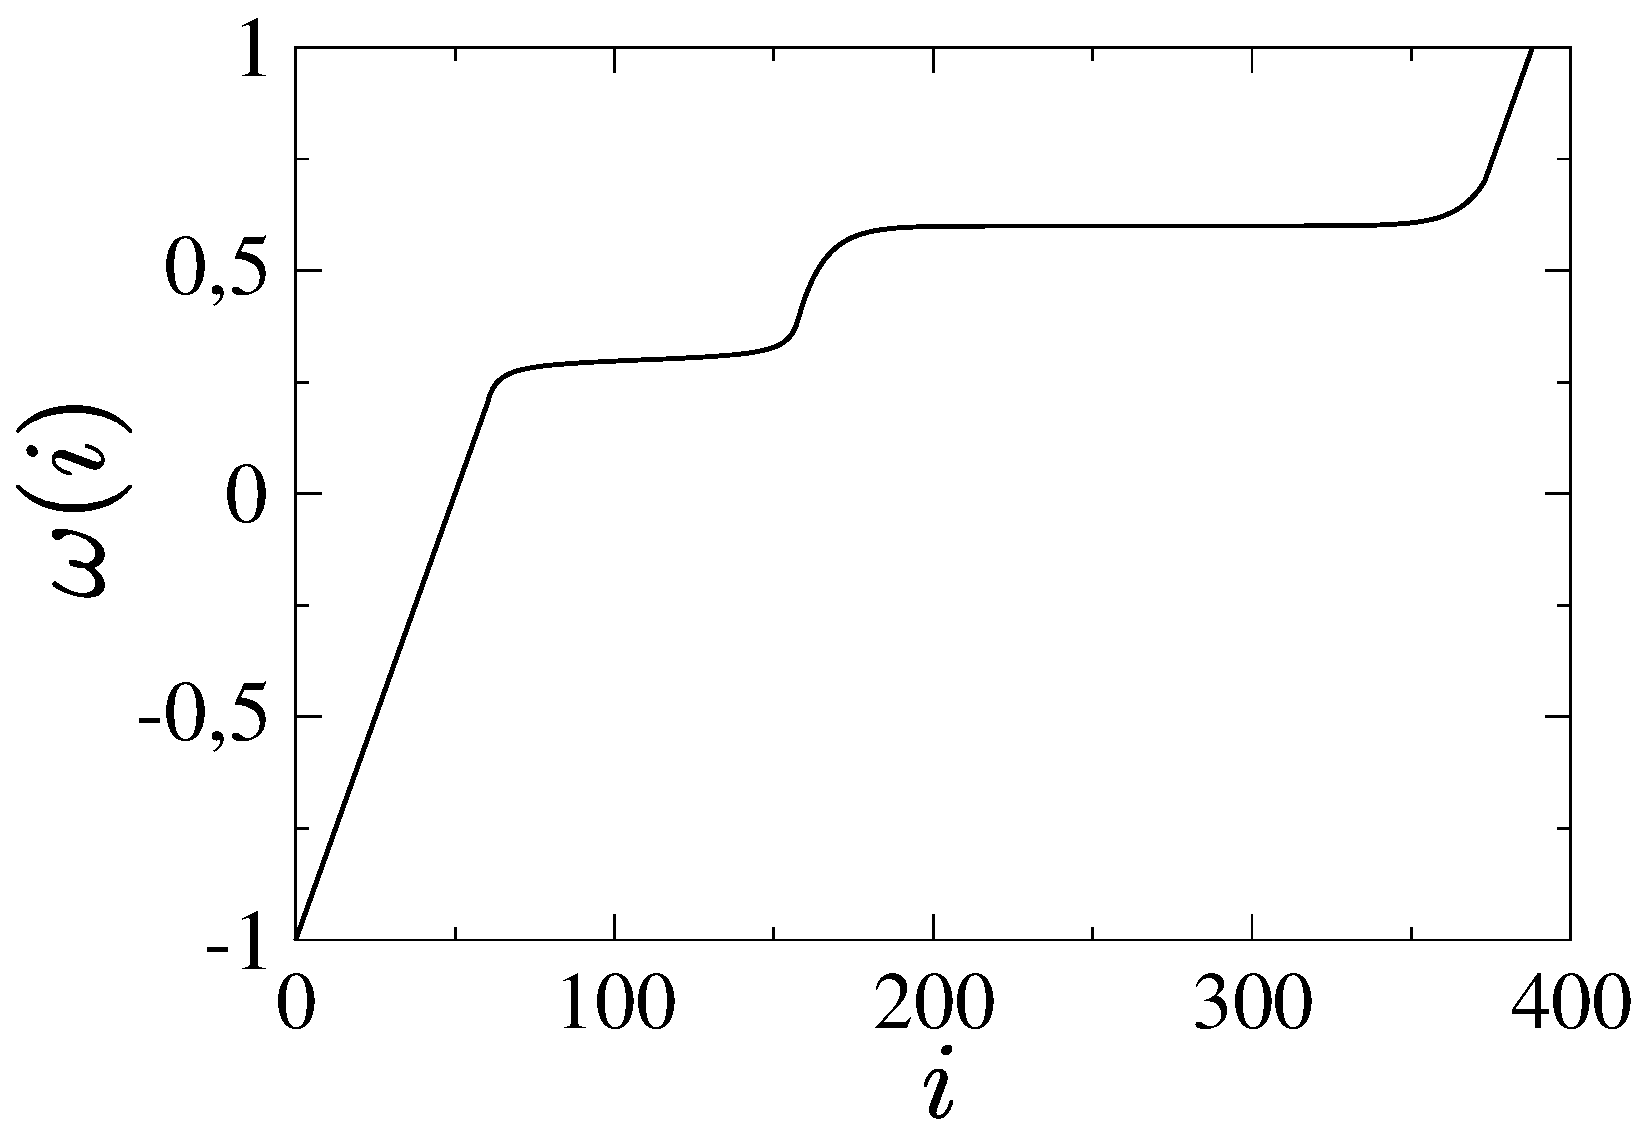
\includegraphics[width=0.5\textwidth]{pics/example_add_gr.eps}
	\caption{Multigrid corresponding to listing \ref{lst:add_gr}}
	\label{fig:example_add_gr}
\end{figure}

\begin{lstlisting}[caption={Example for replacing a grid region},label={lst:replace_gr}]
mgrid.replace_gr_equi(100, -0.5, 0.0, "gr");
mgrid.create();
\end{lstlisting}

In listing \ref{lst:replace_gr} the logarithmic grid region named ``gr'' from the multigrid instance ``mgrid'' is replace by an equidistant grid region with the same name. In order to apply this change the create function has to be invoked once again. Note, that if one tries to replace a non-existing grid region, this will result in a simple adding of the desired grid region. The resulting multigrid is shown in figure \ref{fig:example_replace_gr}.
\begin{figure}[h]
	\centering
	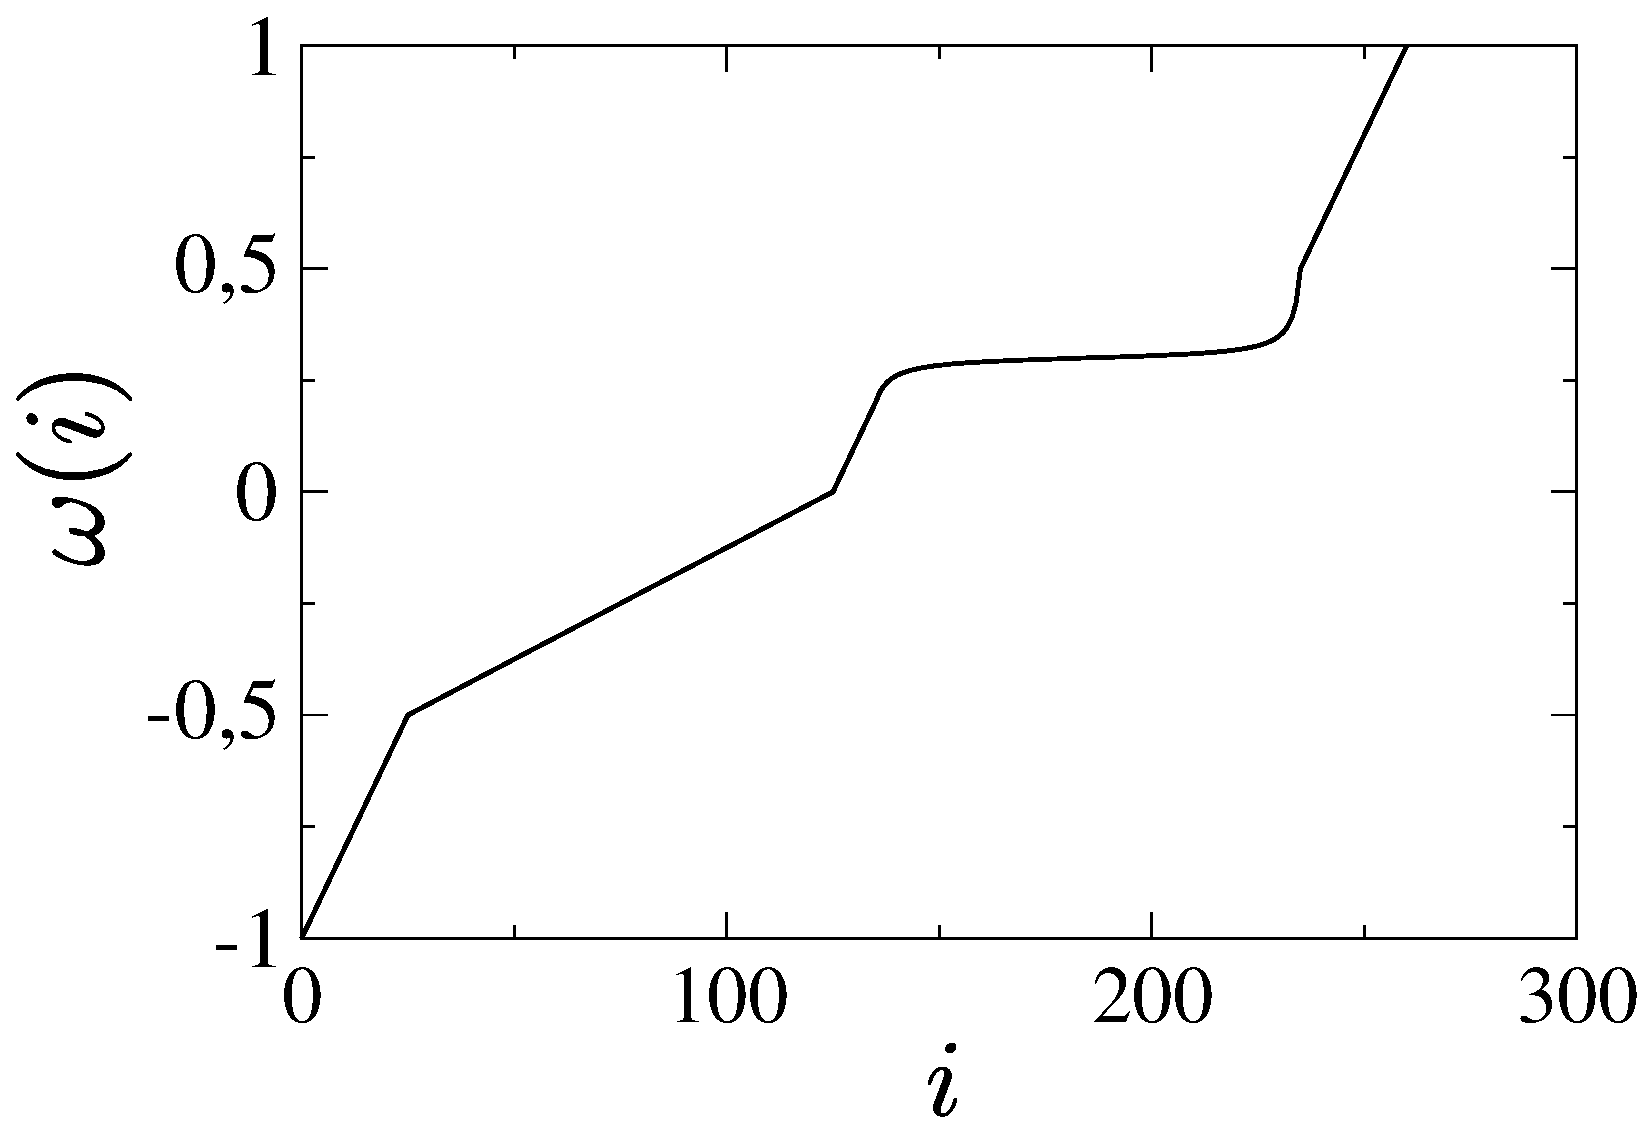
\includegraphics[width=0.5\textwidth]{pics/example_replace_gr.eps}
	\caption{Multigrid corresponding to listing \ref{lst:replace_gr}}
	\label{fig:example_replace_gr}
\end{figure}

\subsection{More convenient ways of adding and replacing}\label{subsec:wrapper}
There are more convenient ways of adding or replacing equidistant and logarithmic grid regions. For the former it might be desirable to specify the grid resolution $d\omega$ instead of the number of grid points $M$. And for the latter it would be convenient just to give the maximal resolution at the center point $d\omega_{min}$ and the minimal resolution at the boundaries $d\omega_{max}$ together with the center point $\omega_k$ and the half width of the grid region $\omega_1=(\omega_r-\omega_l)/2$ instead of specifying the grid point numbers $N_l$ and $N_r$, $\omega_0$ and the boundaries $\omega_l$ and $\omega_r$. Note that hereby we made the logarithmic grid region symmetric around the center point. There are wrapper functions for adding and replacing equidistant and logarithmic grid regions which possess these properties. They are shown in the tables \ref{tab:add_gr_equi_wrapper} and \ref{tab:add_gr_log_wrapper}. For examples see chapter \ref{chapter:quick_start_guide}, where these wrapper functions are used throughout the entire chapter. Note that the center point of the equidistant grid region is naturally chosen to be $\omega_c=(\omega_r-\omega_l)/2$.

\begin{table}[h]
	\begin{center}
		\begin{tabular}{lll}		
		Argument  & Type & Description \\ \hline
		\nth{1}   & \texttt{double} & Lower boundary ($\omega_l$) \\ 
		\nth{2}   & \texttt{double} & Upper boundary ($\omega_r$) \\ 
		\nth{3}   & \texttt{double} & Resolution ($d\omega$) \\
		(\nth{4}) & \texttt{string} & Name of the grid region (\texttt{id})(optional)\\ 
		\end{tabular}
	\end{center}
	\caption{Arguments of the wrapper functions \texttt{add\_gr\_equi} and \texttt{replace\_gr\_equi}}
	\label{tab:add_gr_equi_wrapper}
\end{table}

\begin{table}[h]
	\begin{center}
		\begin{tabular}{lll}		
		Argument  & Type & Description \\ \hline
		\nth{1}   & \texttt{double} & Center point ($\omega_k$) \\ 
		\nth{2}   & \texttt{double} & Half width ($\omega_1$) \\ 
		\nth{3}   & \texttt{double} & Maximal resolution at the center point ($d\omega_{min}$)\\ 
		\nth{4}   & \texttt{double} & Minimal resolution at the boundaries ($d\omega_{max}$)\\ 
		(\nth{5}) & \texttt{string} & Name of the grid region (\texttt{id})(optional)\\ 
		\end{tabular}
	\end{center}
	\caption{Arguments of the wrapper functions \texttt{add\_gr\_log} and \texttt{replace\_gr\_log}}
	\label{tab:add_gr_log_wrapper}
\end{table}

For the logarithmic grid region the mapping from maximal and minimal resolutions $d\omega_{max}$ and $d\omega_{min}$ to the loggrid variables $\omega_0$, $N_l$ and $N_r$ is determined by the following equations:
\begin{align*}
	\omega_0 & = \frac{\omega_1 d\omega_{min}}{d\omega_{max}}\\
        N_l=N_r& =log\left(\frac{\omega_1}{\omega_0}\right) \frac{\omega_1}{d\omega_{max}}
\end{align*}

\section{Fundamental and special grid regions}\label{sec:fundamental_and_special_grid_regions}
\index{Fundamental grid regions}
\index{Special grid regions}
As it was explained in the beginning of this chapter, the base grid region defines the outer boundaries of the multigrid. A grid region which is added to the multigrid after the base grid region is called fundamental grid region (FGR). The selection and cutting procedure will remove all overlaps between the FGR (see chapter \ref{chapter:multigrid_selection_and_cutting}). By adding such an FGR, all the grid points of the base grid which lie inside the boundaries of the FGR will be removed and replaced by the grid points of the FGR.

Up to now, the base grid has to be one of the grid regions based on the simple grids: equidistant, tangential or logarithmic. But in principle there is nothing to be said against using a multigrid itself as a base grid. This is achieved by letting the basic grid region and the FGR go through the selection and cutting procedure and building a ``multigrid''-like grid which is called the fundamental grid. The fundamental grid serves as a ``base'' grid for additional grid regions which will be called special grid regions (SGR). These special grid regions are added, replaced or removed exactly in the same way as for the FGR. The only difference is, that one has to replace the '\texttt{gr}' in the member functions of section \ref{sec:grid_regions} by a '\texttt{sgr}'.
\begin{lstlisting}[caption={Example for adding special grid regions},label={lst:add_sgr}]
	multigrid mgrid;
	mgrid.add_gr_equi(100, -1, 1, 0);
	mgrid.add_gr_tan(100, 0.2, 0.5, 0.3, 0.01);
	mgrid.add_gr_log(100, 100, 0.4, 0.7, 0.6, 1E-6, "gr");
	mgrid.add_sgr_equi(0.5, 0.8, 0.001);
	mgrid.create();
\end{lstlisting}
Listing \ref{lst:add_sgr} is exactly the same as listing \ref{lst:add_gr} but with an additional adding of a special equidistant grid region from $0.5$ to $0.8$ with resolution $0.001$. (Note, that we used one of the wrapper functions from section \ref{subsec:wrapper} here.) This SGR will just ``bump away'' most parts of the logarithmic grid region, even though its maximal resolution ($10^{-6})$ is much higher than the one of the SGR ($10^{-4}$). Therefore one can use SGR for ``tricking'' the selection and cutting procedure to some extent. It is needless to say, that if you add multiple SGR they will also run through a selection and cutting procedure. The resulting multigrid of listing \ref{lst:add_sgr} is shown in figure \ref{fig:example_add_sgr}.
\begin{figure}[h]
	\centering
	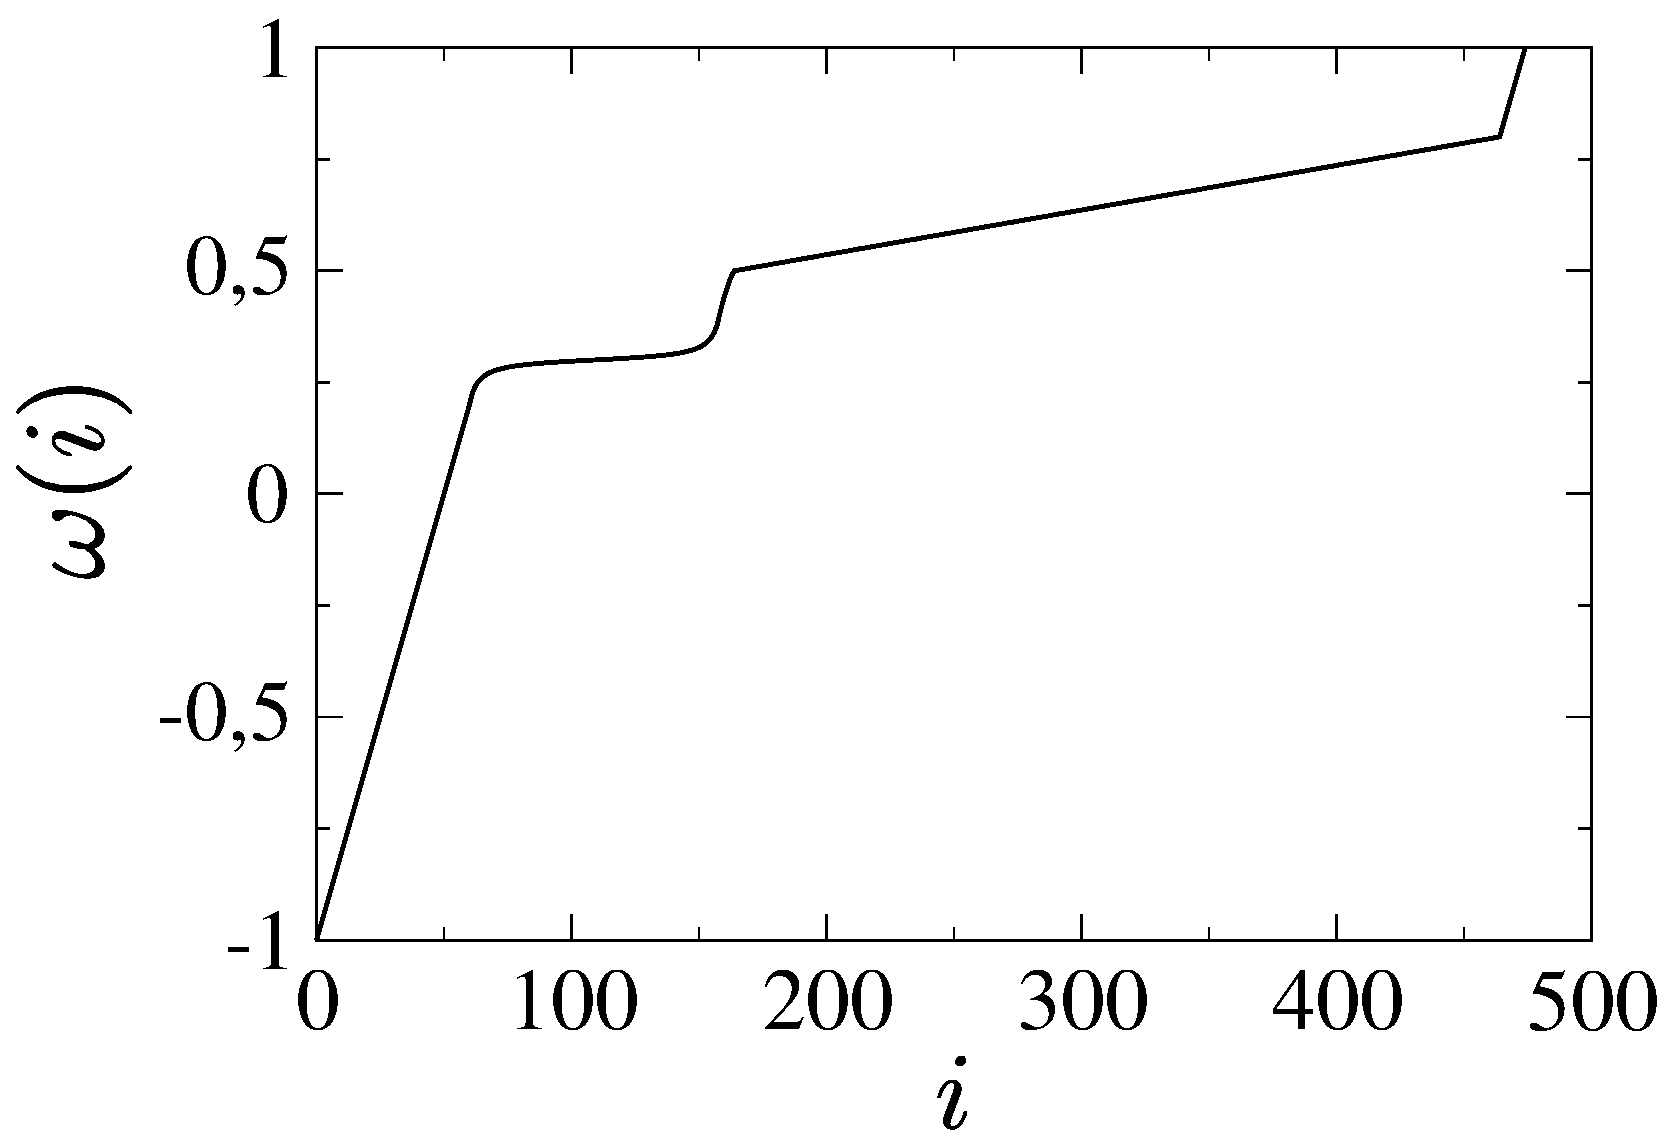
\includegraphics[width=0.5\textwidth]{pics/example_add_sgr.eps}
	\caption{Multigrid corresponding to listing \ref{lst:add_sgr}}
	\label{fig:example_add_sgr}
\end{figure}


\chapter{Selection and Cutting in the Multigrid} \label{chapter:multigrid_selection_and_cutting}
In this chapter the details of the selection and cutting procedure will be explained. Moreover, we will show how to keep track of the inverse mapping while adding fundamental and special grid regions to the multigrid. For the sake of clarity, we will ignore the special grid regions in most parts of this chapter and come back to them in the last part of this chapter.
\section{Cutting procedure}\label{sec:cutting_procedure}
\index{Cutting procedure}
As it was shown in the last chapter, each grid region has a center point $\omega_c$, a buffer region boundary below and above the center point $d\omega_-$ and $d\omega_+$, and an upper and lower boundary $\omega_l$ and $\omega_r$. If there is any overlap between two grid regions, the boundaries and grid parameters have to be adapted such, that the resolution remains constant across the cutting point. We consider two overlapping grid regions and indicate the grid region with the smaller center point by a superscript $l$ for left, and the other one by a superscript $r$ for right (see figure \ref{fig:cutting_gr}).

\begin{figure}[h]
	\centering
	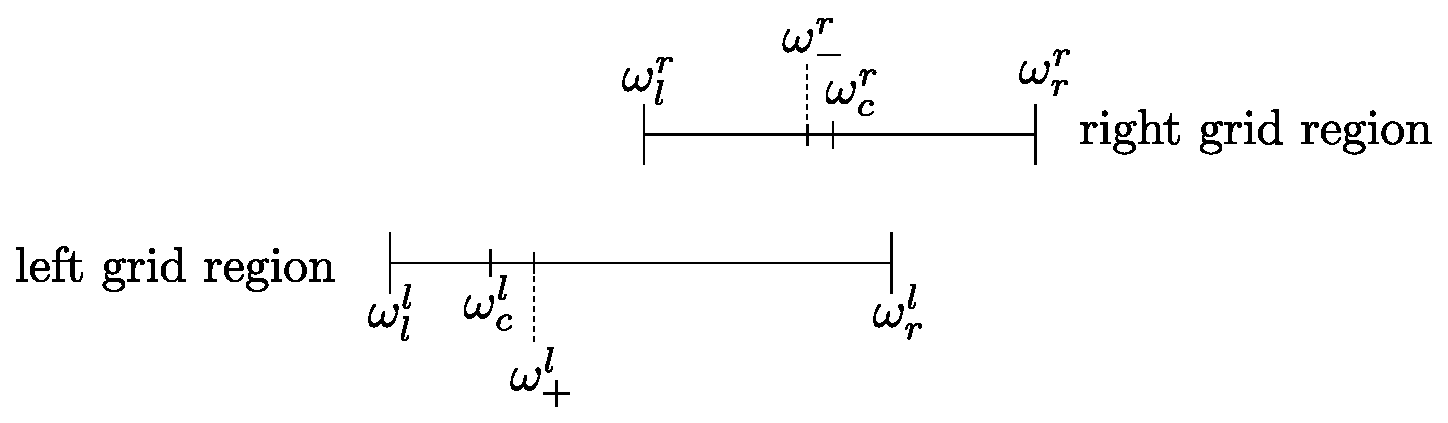
\includegraphics[width=0.8\textwidth]{pics/cutting_gr.eps}
	\caption{Nomenclature for the cutting of two intersecting grid regions}
	\label{fig:cutting_gr}
\end{figure}

The cutting point must be right from the center point of the left grid region plus a small grid dependent buffer, this point is $\omega_+^l$. It also has to be left from the center point of the right grid region minus a small grid dependent buffer, this point is $\omega_-^r$. Moreover the cutting point must not exceed the right boundary of the left grid region $\omega_r^l$ while at the same time it must not fall below the left boundary of the right grid region $\omega_l^r$. Therefore the cutting point $\omega_s$ must lie inside the interval
\begin{equation}\label{eqn:cutting_point_boundaries}
	\omega_s \in [\,max(\omega_+^l, \omega_l^r)\,,\;\; min(\omega_-^r, \omega_r^l)\,]\;:=I
\end{equation}
In this interval, the grid point density of the left grid region $\frac{di}{d\omega}|_l$ is monotonically decreasing and the grid point density of the right grid region $\frac{di}{d\omega}|_r$ is monotonically increasing. The cutting point should be that point, where the grid point densities of both grid regions become equal
\begin{equation}\label{eqn:cutting_point}
	\left. \frac{di}{d\omega}\right|_l(\omega_s) \stackrel{!}{=} \left. \frac{di}{d\omega}\right|_r(\omega_s)
\end{equation}
This equation, can be solved analytically for all combinations of equidistant, tangential and logarithmic grid regions. This is done in appendix \ref{sec:app_cutting_points}. The calculated cutting point does not always lie inside the interval $I$. In such a case one has to put more thought in what to do. This is done in the following where we list all possibilities which can occur if a solution to equation \ref{eqn:cutting_point} exists (see also figure \ref{fig:cutting_gr_cases}):

\begin{itemize} % itemize because cases label should be in agreement with source code
	\item{\bf Case A}: $\omega_s \in I$: If the calculated cutting point lies inside the interval $I$, both grids are cut at this particular point.

	\item{\bf Case B}: $\omega_s \notin I$ and $\omega_s \in [\omega_l^r, \omega_+^l)$ and $\omega_s \notin (\omega_-^r, \omega_r^l]$: This means, that the maximal resolution of the left grid is smaller than the resolution of the right grid at $\omega_+^l$. Therefore the purpose of the left grid region is assumed to be fulfilled by the right grid region, and the left grid region is skipped.

	\item{\bf Case C}: $\omega_s \notin I$ and $\omega_s \notin [\omega_l^r, \omega_+^l)$ and $\omega_s \in (\omega_-^r, \omega_r^l]$: This means, that the maximal resolution of the right grid is smaller than the resolution of the left grid at $\omega_-^r$. Therefore the purpose of the right grid region is assumed to be fulfilled by the left grid region, and the right grid region is skipped.

	\item{\bf Case D}: $\omega_s \notin I$ and $\omega_s \in [\omega_l^r, \omega_+^l)$ and $\omega_s \in (\omega_-^r, \omega_r^l]$: The distance between both center points is so small, that the calculated cutting point lies inside both buffer regions. Here, the grid region with the smaller maximal resolution is skipped.

	\item{\bf Case E}:  $\omega_s \notin I$ and $\omega_s < \omega_l^r$. The resolution of the right grid region is greater than the resolution of the left grid region over the whole range of the right grid region, even at $\omega_l^r$. Therefore the right grid region will not be cut at all. If there is still enough space for the left grid region, i.e. if $\omega_+^l\leq\omega_l^r$, the left grid region will be cut at $\omega_l^r$. If not, the left grid region will be skipped.

	\item{\bf Case F}:  $\omega_s \notin I$ and $\omega_s > \omega_r^l$. The resolution of the left grid region is greater than the resolution of the right grid region over the whole range of the left grid region, even at $\omega_r^l$. Therefore the left grid region will not be cut at all. If there is still enough space for the right grid region, i.e. if $\omega_-^r \geq \omega_r^l$, the right grid region will be cut at $\omega_r^l$. If not, the right grid region will be skipped.
\end{itemize}

\begin{figure}[h]
	\centering
	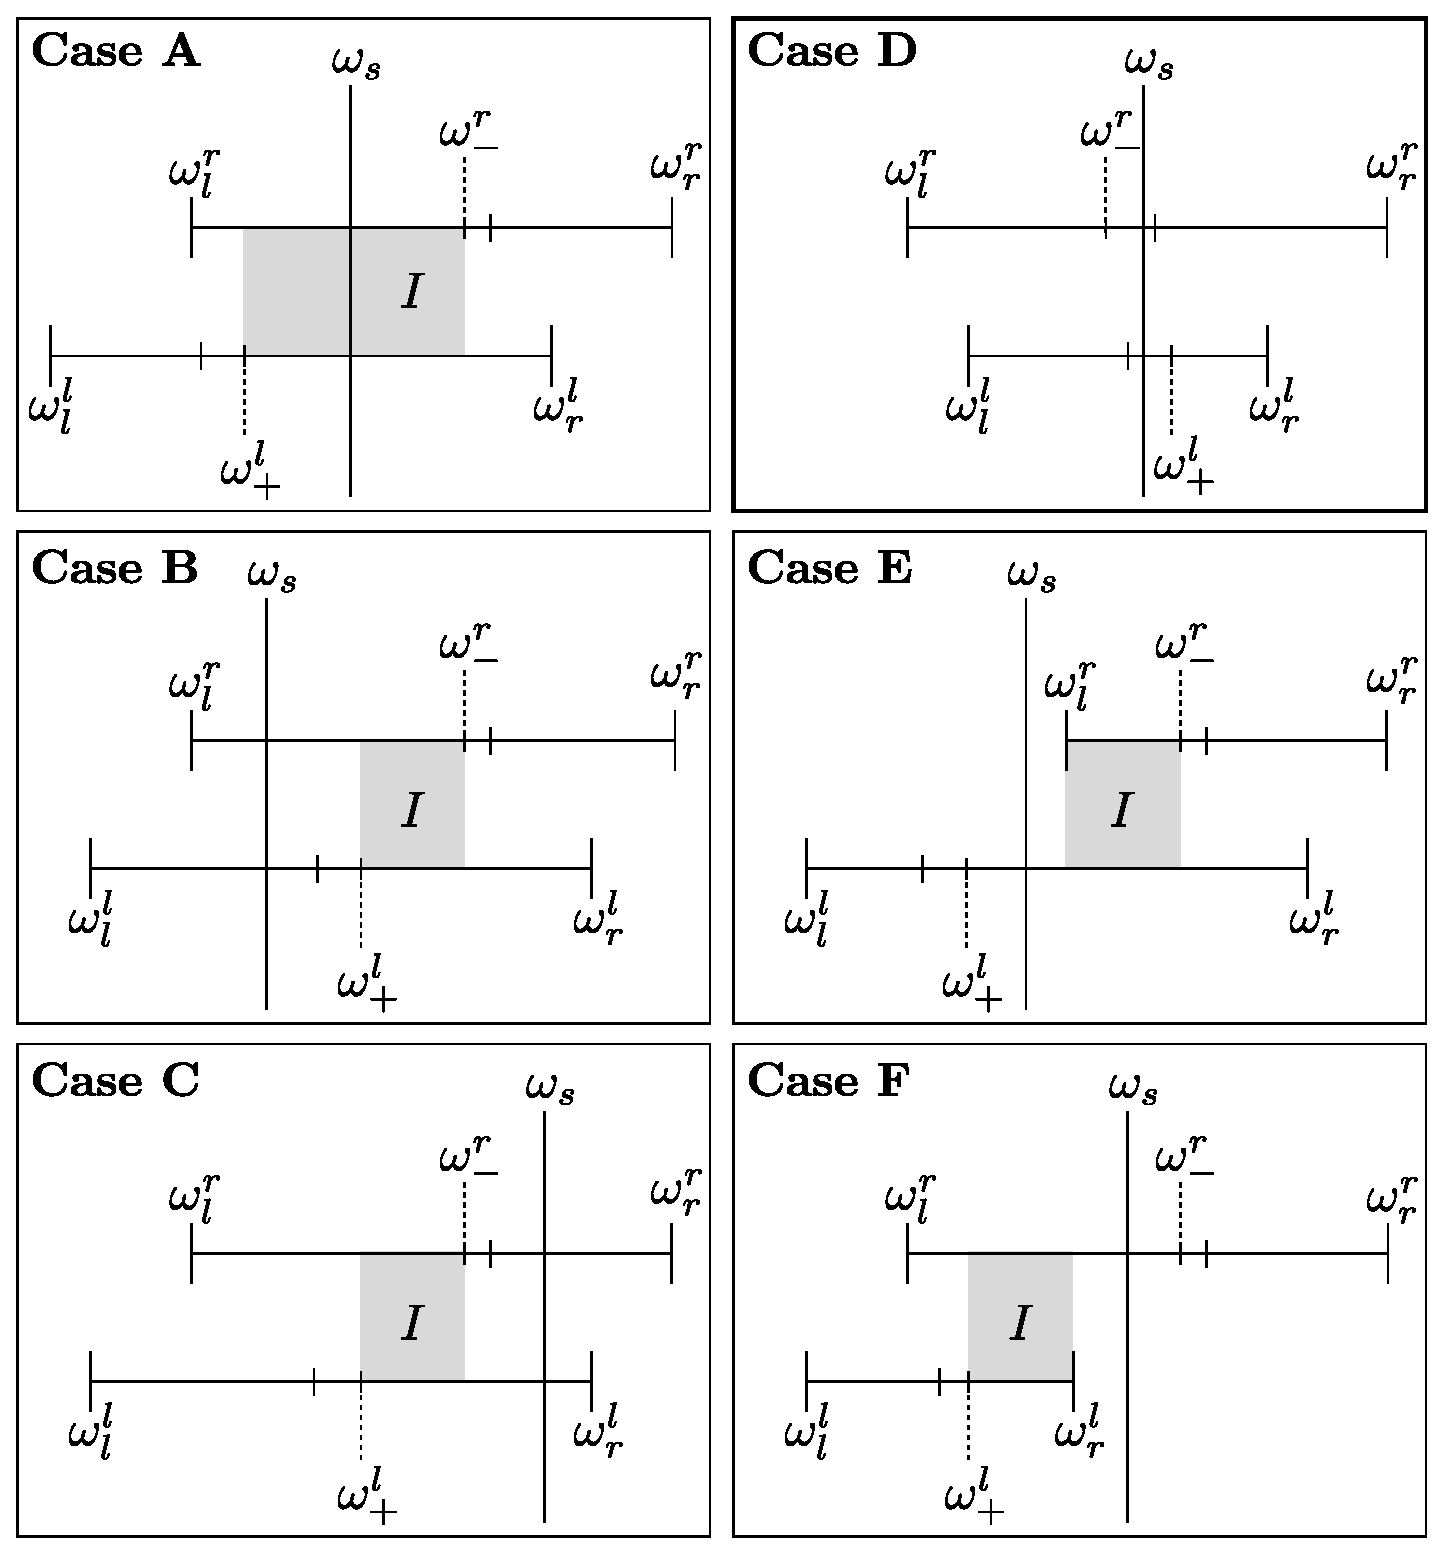
\includegraphics[width=0.8\textwidth]{pics/cutting_gr_cases.eps}
	\caption{Different cases for the cutting of two overlapping grid regions}
	\label{fig:cutting_gr_cases}
\end{figure}

Of course there are cases, in which a solution to equation \ref{eqn:cutting_point} does not exist. If this happens, the lowest resolution of one grid region is higher than the highest resolution of the other. This is basically the same situation as in the cases E and F in the above listing. The only difference is, that one has to find out which of the both grid regions should be favored. This is done by comparing the maximal resolution of both grid regions. Afterwards, one checks if there is still enough space for the non-favored grid region. If this is the case, it will be cut, otherwise it will be skipped  (see cases E and F).

By cutting a grid region at a given cutting point, one has to adjust the grid parameter of this grid region such, that the maximal resolution remains the same. This adaption is different for the equidistant, tangential and logarithmic grid regions and is explained in appendix \ref{sec:app_cutting_gr}.

Grid regions which have overlap with the boundaries of the basic grid region are selected and cut in a similar way. If the center point is outside of these boundaries, the grid region is skipped. It is also skipped if there is not enough space between the buffer region and the boundaries (like in the cases E and F). Otherwise it is cut at the boundaries.

So far, we have only considered two overlapping grid regions. We have shown how the selection and cutting procedure works in this case. Treating multiple overlapping grid regions is a bit more complicated, but can be boiled down to the two grid region case in the end. We will show how this is done in the following. At first, all grid regions are sorted with respect to their center points. Afterwards one iterates through all neighboring pairs of grid regions, starting from the left, i.e. the grid region with the lowest center point, and applies the selection and cutting procedure to each of these pairs. If none of both grid regions is decided to be skipped, the algorithm proceeds to the next pair of neighboring grid regions. Otherwise, if one of the grid regions has to be skipped, it is necessary to re-evaluate all the pairings to the left of this grid region. Therefore the algorithm erases this particular grid region and restarts the iterating pair selection and cutting procedure, which was described above, again from the far left. This is continued until the most right grid region pair is reached.



\section{Subgrids and inserting grid regions}\label{sec:subgrids_and_insert}
\index{Subgrid}
\index{Inverse of the multigrid}
If all fundamental grid regions have gone through the cutting procedure explained in \ref{sec:cutting_procedure}, we are left with a bunch of non-intersection grid regions. These grid regions are now ready to be inserted into the basic grid region. There is one difficulty we have not mentioned so far: One has to take care of the inverse. Since all grid regions consist of one of the simple grid classes from chapter \ref{chapter:simple_grids}, their inverse mapping is known. For the same reason, we know the inverse of the basic grid region. In order to calculate the inverse of the resulting multigrid, one has to keep track of the indices at which the non-overlapping grid regions are inserted. We will show how this is done in the following. First of all it will turn out to be useful to introduce the notion of a subgrid, and the corresponding \texttt{subgrid} class. 

\begin{table}[h]
	\begin{center}
		\begin{tabular}{ll}
		Name & Description \\ 
		\hline
		$\omega_l$  & Lower boundary \\
		$\omega_r$  & Upper boundary \\
		$i_l$       & Lower index cut region in basic grid \\
		$i_r$       & Upper index cut region in basic grid \\
		$N_R$       & Difference in overall grid points before and after insertion \\
		\texttt{type}  & Type of subgrid (equi, tan or log)\\
		$\dots$ & Grid region parameters (e.g. $\omega_k$ and $\omega_0$ for the loggrid) \\
		\end{tabular}
	\end{center}
	\caption{Properties of the subgrid}
	\label{tab:subgrid}
\end{table}

In table \ref{tab:subgrid} the properties of the subgrid class are shown. Like a grid region, a subgrid contains the information about the boundaries and the type of grid it contains. It does not contain any information about the center point or the resolution since the cutting and selection procedure has already been performed. But it stores information about the inserting of the subgrid into the basic grid region, i.e. the lower and upper index of the region which will be cut out of the basic grid $i_l$ and $i_r$, and the difference in the overall number of grid points before and after the insertion $N_{R}$. 

The most decisive property of a subgrid is, that there is no overlap between different subgrids (in contrast to grid regions). After applying the selection and cutting procedure to the grid regions they will not have any overlap, too. Therefore all grid regions can be mapped to subgrids. After this is done, the subgrids can be inserted into the basic grid. In the following, we will show how a subgrid $\epsilon(i)$ of length $N$ with boundaries $\epsilon_l$ and $\epsilon_r$ is inserted into a basic grid $\omega(i)$ of length $M$ (see figure \ref{fig:subgrid_inserting}). 

\begin{figure}[h]
	\centering
	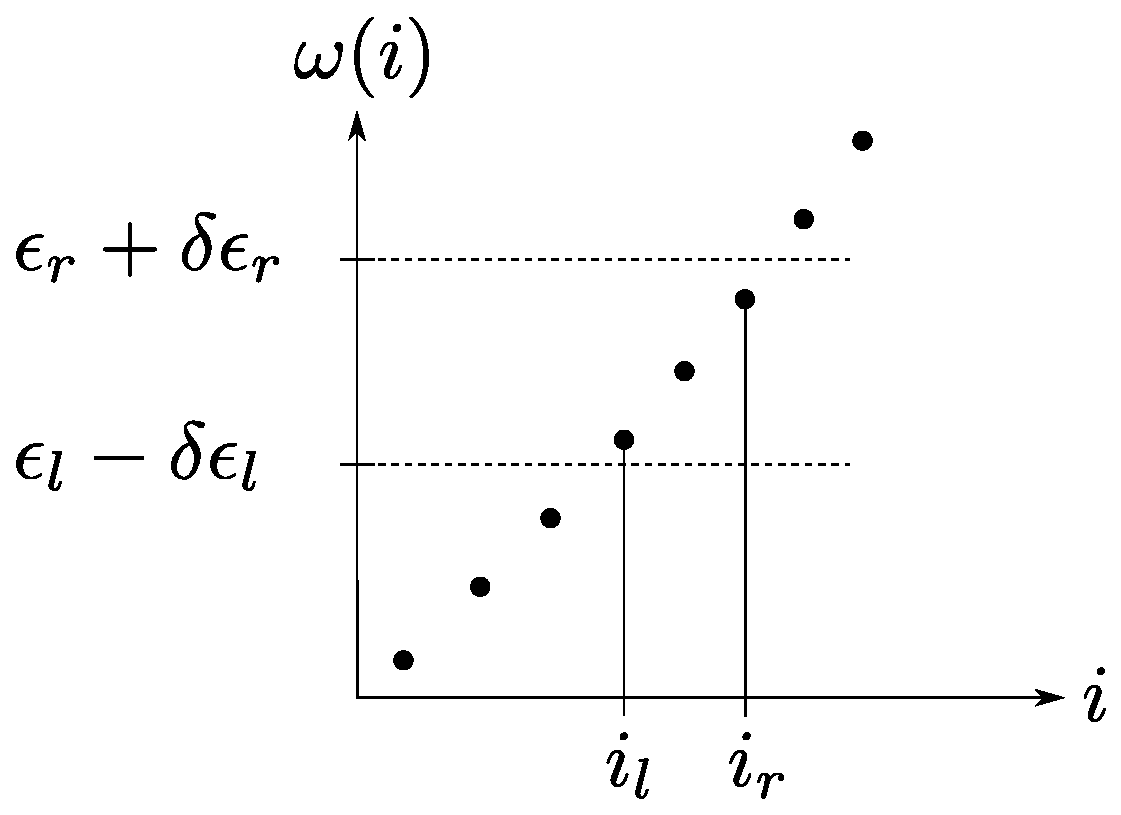
\includegraphics[width=0.4\textwidth]{pics/subgrid_inserting.eps}
	\caption{Inserting of a subgrid}
	\label{fig:subgrid_inserting}
\end{figure}
The indices $i_l$ and $i_r$ are obtained by
\begin{align*}
	\omega(i_l) & > \epsilon_l - \delta \epsilon_l \quad \text{with } i_l \text{ minimal} \\
	\omega(i_r) & < \epsilon_r + \delta \epsilon_r \quad \text{with } i_r \text{ maximal} \\
\end{align*}
where the machine precision buffer $\delta$ ensures that the resulting grid point difference ($\sim$~weights) does not become too small. 
The difference in the overall grid point number is then given by
\[
	N_R=N +1 - (i_r-i_l+1)
\]
The subgrid is inserted into the base grid at the index $i_l$. The resulting grid $\tilde \omega(i)$ is then given by
\[
	\tilde \omega(i)=\begin{cases}
			\omega(i) \quad & i = 0,\dots,i_l-1 \\
			\epsilon(i-i_l) \quad & i=i_l,\dots,i_l+N\\
			\omega(i-N_R) \quad & i=i_l+N+1,\dots,M+N_R
 	          \end{cases}
\]
The grid $\tilde \omega(i)$ then serves as a basic grid for the insertion of the next subgrid. Nevertheless if there is more than one subgrid, there is an additional subtlety which has to be taken into account: If one inserts a subgrid left from a subgrid which was inserted earlier, one has to shift the indices $i_l$ and $i_r$ for the latter one by the number of replaced grid points $N_R$ of the former one. This means, that if one adds a subgrid with $N_R^\text{new}$, one has to shift the indices $i_l$ and $i_r$ of all subgrids which lie right of the former one by
\begin{align*}
	i_l &\to i_l + N_R^\text{new} \\
	i_r &\to i_r + N_R^\text{new} \\
\end{align*}
By this procedure the multigrid is build up out of several subgrids and the basic grid.

\section{Inverse of the multigrid}\label{sec:inverse_of_the_multigrid}
\index{Inverse of the multigrid}
In this section we will show how to calculate the inverse $i(\omega)$ of a multigrid which consists of a basic grid and several subgrids. As an example we take the multigrid from listing \ref{lst:replace_gr}, see figure \ref{fig:inverse}.

\begin{figure}[h]
	\centering
	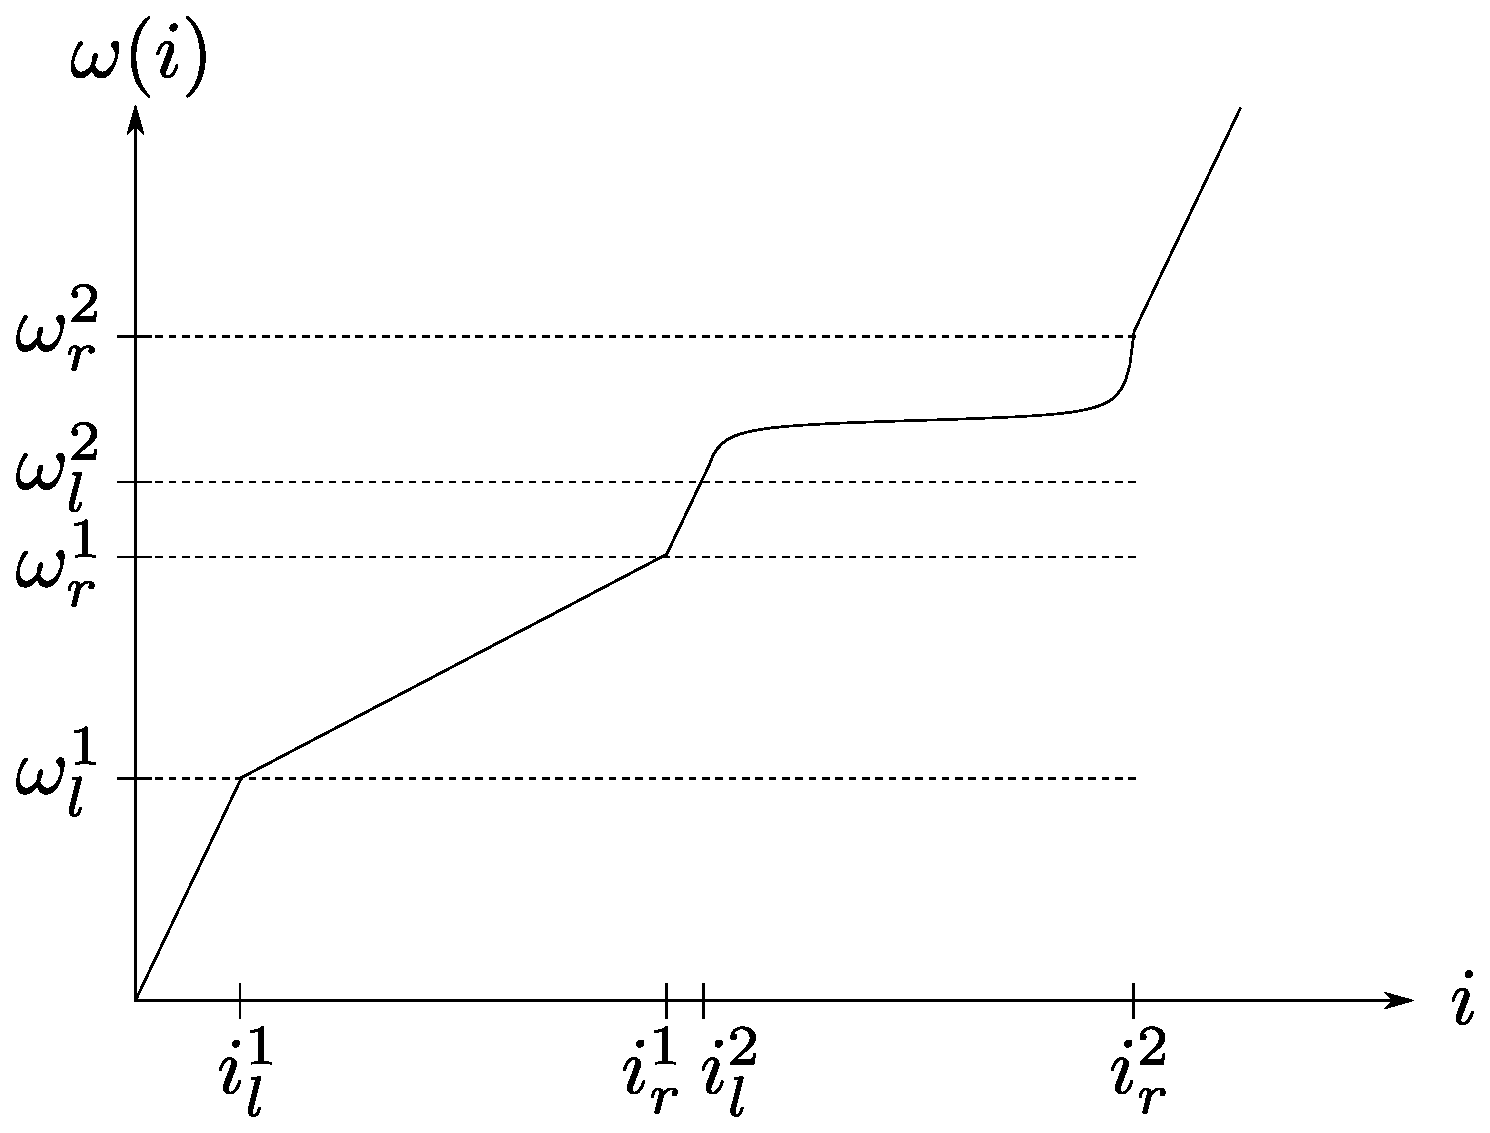
\includegraphics[width=0.5\textwidth]{pics/inverse.eps}
	\caption{Calculating the inverse mapping of a multigrid}
	\label{fig:inverse}
\end{figure}

There is an equidistant basic grid and two subgrids, an equidistant and a tangential one. We will denote the basic grid by $\omega^0(i)$, the equidistant subgrid by $\omega^1(i)$ and the tangential subgrid by $\omega^2(i)$. The corresponding inverse mappings are denoted by $i^0(\omega)$ for the basic grid, $i^1(\omega)$ for the equidistant subgrid and $i^2(\omega)$ for the tangential subgrid. In order to calculate the inverse of a given value $\omega$ one has to find out, if $\omega$ lies in one of the subgrid regions. And if this is the case, in which subgrid. Otherwise, one uses the inverse of the basic grid $i^0(\omega)$. The resulting inverse mapping is then given by
\begin{equation}\label{eqn:inverse}
	i(\omega)=\begin{cases}
			i^1(\omega) + i_l^1 \quad & \omega \in [\omega_l^1, \omega_r^1]\\
			i^2(\omega) + i_l^2 \quad & \omega \in [\omega_l^2, \omega_r^2]\\
			i^0(\omega) + N_S \quad & \omega \notin [\omega_l^1, \omega_r^1] \cup [\omega_l^2, \omega_r^2]
	          \end{cases}
\end{equation}
Where $N_S$ is the sum of all numbers of replaced points $N_R^k$ which correspond to subgrids $k$, which are left of $\omega$, i.e. which fulfill $\omega_r^k<\omega$:
\[
	N_S=\sum_{\substack{k\\ \omega_r^k<\omega}} N_R^k
\]
The generalization to an arbitrary number of subgrids is straight forward. Now it is clear, why the subgrids contain $i_l$ and $N_R$: they are directly used in the calculation of the inverse mapping.

\section{Fundamental and special grid regions}\label{sec:fundamental_and_special_grid_regions_2}
\index{Fundamental grid regions}
\index{Special grid regions}
The above multigrid was comprised of a basic grid and several subgrids. Up to now these subgrids were build out of fundamental grid regions. Therefore they are so-called fundamental subgrids and we will call the resulting grid a fundamental grid. In the last section we have shown how to calculate the inverse of such a fundamental grid. Nothing prevents us from taking this fundamental grid as a basic grid for inserting more subgrids. In accordance to the special grid regions introduced in the last chapter, we will call them special subgrids. After the selection and cutting procedure the special grid regions are mapped onto special subgrids. In the same way the fundamental subgrids were inserted into the basic grid to form the fundamental grid, the special subgrids are inserted into the fundamental grid to form the resulting multigrid. While calling the inverse of a value $\omega$ of a multigrid, the algorithm  will begin by checking weather $\omega$ is inside one of the special subgrids (just like for the fundamental subgrids in equation \ref{eqn:inverse}). If this is the case it will calculate the inverse mapping of the subgrids directly (again, just like in equation \ref{eqn:inverse}). Otherwise it will call the inverse mapping of the fundamental grid (just like the inverse of the basic grid $i^0(\omega)$ is called in \ref{eqn:inverse}). The calculation of the inverse of the fundamental grid was explained in the last sections.




\chapter{Mesh - Multigrid without Inverse Mapping}
There might be occasions where the inverse mapping of the multigrid is not needed. The mesh grid class is exactly the same as the multigrid class, but without the inverse mapping. All multigrid commands also work for the mesh class. For example 
\begin{lstlisting}
	mesh mgrid;
	mgrid.add_gr_equi(100, -1, 1, 0);
	mgrid.add_gr_tan(100, 0.2, 0.5, 0.3, 0.01);
	mgrid.add_gr_log(100, 100, 0.4, 0.7, 0.6, 1E-6, "gr");
	mgrid.add_sgr_equi(0.5, 0.8, 0.001);
	mgrid.create();
\end{lstlisting}
is exactly the same as listing \ref{lst:add_sgr}, except for the first line. Note that the mesh class is not optimized for fast initialization since internally, the mesh \texttt{create} function will call the multigrid \texttt{create} function, which takes care of all the subgrid indices needed for the inverse mapping.

In comparison to the multigrid, there are only two additional features, which at the same time destroys the possibility of calculating the inverse of a mesh. The first one is the adding of single points inside grid by
\texttt{add\_spoint}. The second one is the adding of terminating points which serve as the total upper and lower boundary of the mesh by \texttt{add\_lendpoint} for the lower endpoint and \texttt{add\_rendpoint} for the upper endpoint. Hereby it is possible to cut of a multigrid at arbitrary points for the prize of giving up the possibility of calculating an inverse mapping. Listing \ref{lst:mesh} shows an example for an instance of the mesh class.
\begin{lstlisting}[caption={Example of a mesh},label={lst:mesh}]
mesh amesh;
amesh.add_gr_equi(10, 0.0, 1, 0.5);
amesh.add_gr_log(0.75, 0.1, 1E-1, 1E-2);
amesh.add_spoint(0.76);
for (int j=0; j!=100; j++)
{
	amesh.add_spoint(0.6+j/100.0);
}
amesh.add_lendpoint(0.15);
amesh.add_rendpoint(0.85);
amesh.create();
\end{lstlisting}
Note, that by inserting a point it will always be taken care of not letting the grid point difference ($\sim$ weights) getting to small (beyond machine precision). This is achieved by skipping all existing points which are to narrow to the inserted point.
\appendix
\chapter{Loggrid parameter}
\section{Boundary conditions}
\label{sec:app_loggrid_boundary}
In the following we will show how the four boundary conditions (\ref{eqn:loggrid_boundary_conditions})
\begin{align}
	\omega(0)&=\omega_{min}   \label{eqn:loggrid_boundary_condition_1}\\
	\omega(N_l-1)&=\omega_k-\omega_0  \label{eqn:loggrid_boundary_condition_2}\\
	\omega(N_l+N_k)&=\omega_k+\omega_0   \label{eqn:loggrid_boundary_condition_3}\\
	\omega(N_l+N_k+N_r)&=\omega_{max}   \label{eqn:loggrid_boundary_condition_4}
\end{align}
determine the four parameters $i_1$, $i_2$, $c_1$ and $c_2$ in the definition of the logarithmic grid~(\ref{eqn:loggrid_definition}):
\begin{equation*}
	\omega(i)=\begin{cases}
		-\exp(-c_1(i-i_1)) + \omega_k 		\quad & i\in\{0,\dots,N_l-1\} \\ 
		\omega_k-\omega_0+d\omega_k(i-N_l)	\quad & i\in\{N_l,\dots,N_l+N_k-1\} \\ 
		\exp(c_2(i-i_2-N_l-N_k)) + \omega_k 	\quad & i\in\{N_l+N_k,\dots,N_l+N_k+N_r\}
	\end{cases}
\end{equation*}

\vspace{1cm}
\noindent\underline{Determine $i_1$ and $c_1$:}\\

\noindent Insert \ref{eqn:loggrid_definition} into (\ref{eqn:loggrid_boundary_condition_1}) and (\ref{eqn:loggrid_boundary_condition_2}):
\begin{align}
	-\exp(-c_1(0-i_1))+\omega_k&=\omega_{min} \quad \Leftrightarrow \quad \log(\omega_k-\omega_{min})=c_1 i_1 \label{eqn:app_loggrid_boundary_condition_1_1}\\
	-\exp(-c_1(N_l-1-i_1))+\omega_k&=\omega_k-\omega_0 \quad \Leftrightarrow \quad \log(\omega_0)=-c_1(N_l-1-i_1) \label{eqn:app_loggrid_boundary_condition_2_1}
\end{align}
Difference (\ref{eqn:app_loggrid_boundary_condition_1_1}) $-$ (\ref{eqn:app_loggrid_boundary_condition_2_1}):
\[
	\log\left(\frac{\omega_k-\omega_{min}}{\omega_0}\right)=c_1 (N_l-1) \quad \boxed{\Rightarrow c_1=\frac{\log\left(\frac{\omega_k-\omega_{min}}{\omega_0}\right)}{N_l-1}}
\]
Insert into (\ref{eqn:app_loggrid_boundary_condition_2_1}):
\[
	\boxed{i_1=\frac{\log(\omega_k-\omega_{min})}{c_1}}
\]

\newpage
\vspace{1cm}
\noindent\underline{Determine $i_2$ and $c_2$:}\\

\noindent Insert \ref{eqn:loggrid_definition} into (\ref{eqn:loggrid_boundary_condition_1}) and (\ref{eqn:loggrid_boundary_condition_2}):
\begin{align}
	\exp(c_2(0-i_2))+\omega_k&=\omega_k+\omega_0 \quad \Leftrightarrow \quad \log(\omega_0)=c_2 (0-i_2) \label{eqn:app_loggrid_boundary_condition_3_1}\\
	\exp(c_2(N_r-i_2))+\omega_k&=\omega_{\max} \quad \Leftrightarrow \quad \log(\omega_{max}-\omega_k)=c_2(N_r-i_2) \label{eqn:app_loggrid_boundary_condition_4_1}
\end{align}
Difference (\ref{eqn:app_loggrid_boundary_condition_4_1}) $-$ (\ref{eqn:app_loggrid_boundary_condition_3_1}):
\[
	\log\left(\frac{\omega_{max}-\omega_k}{\omega_0}\right)=c_2 (N_r)\\\Rightarrow \boxed{c_2=\frac{\log\left(\frac{\omega_{max}-\omega_k}{\omega_0}\right)}{N_r}}
\]
Insert into (\ref{eqn:app_loggrid_boundary_condition_4_1}):
\[
	\boxed{i_2=-\frac{\log(\omega_{max}-\omega_k)}{c_2} + N_r}
\]
\section{Maximal resolution}
\label{sec:app_loggrid_max_resolution}
The maximal resolution of the exponential grid regions to the left (region I), $d\omega_{min}^{l}$ and to the right (region III), $d\omega_{min}^{r}$ of the center point in a logarithmic grid reads
\begin{align*}
	d\omega_{min}^{l} & = \omega(N_l-1)-\omega(N_l-2) \notag \\
	& = -\exp(-c_1(N_l-1-i_1))+exp(-c_1(N_l-2-1_1)) \notag \\
	& = \exp(-c_1(N_l-1-i_1))(e^{c_1}-1)
\end{align*}
and
\begin{align*}
	d\omega_{min}^{r} & = \omega(N_l+N_k+1)-\omega(N_l+N_k) \notag \\
	& = \exp(-c_2 i_2)(e^{c_2}-1)
\end{align*}
The resolution of the linear grid (region II) will be the minimum of both
\[
	d\omega_k = min( d\omega_{min}^{l} ,\,d\omega_{min}^{r})
\]
\chapter{Cutting grid regions}\label{chapter:app_cutting}
\index{Cutting points}
\section{Calculation of cutting points}\label{sec:app_cutting_points}
In this section we will calculate the points of equal grid point density $\omega_s$ between two grids of equidistant, tangential and logarithmic type. We will use the corresponding equations for the grid point density of these grid types, i.e.~equations \ref{eqn:equigrid_grid_point_density}, \ref{eqn:tangrid_grid_point_density} and \ref{eqn:loggrid_grid_point_density} in order to solve equation \ref{eqn:cutting_point}. We will go through all possible combinations for the left and right grid region, where we denote the left grid region parameters by a superscript $l$ and the right grid region parameter by a superscript $r$.
\begin{enumerate}
	\item {\bf loggrid/loggrid}:
		\begin{align*}
			\frac{1}{c_2^l(\omega_s-\omega_k^l)}\stackrel{!}{=}\frac{1}{c_1^r(\omega_k^r-\omega_s)}
		\end{align*}
		\[
		 	\Rightarrow \boxed{\omega_s=\frac{c_2^l\omega_k^l + c_1^r\omega_k^r}{c_2^l+c_1^r}}
		\]

	\item {\bf loggrid/tangrid}:
		\begin{align*}
			&\frac{1}{c_2^l(\omega_s-\omega_k^l)}\stackrel{!}{=}\frac{1}{c^r\Delta u^r\left(1+\left(\frac{\omega_s-\omega_c^r}{c^r}\right)^2\right)}\\
			&\Leftrightarrow c_2^l(\omega_s-\omega_k^l) = c^r \Delta u^r + \frac{\Delta u^r}{c^r} (\omega_s-\omega_c^r)^2\\
			&\Leftrightarrow \omega_s^2 - \left(2\omega_c^r + \frac{c^r c_2^l}{\Delta u^r}\right) \omega_s + \left((\omega_c^{r})^2 + (c^r)^2 + \frac{c^r c_2^l}{\Delta u^r} \omega_k^l \right) =0
		\end{align*}
		\[
		 	\Rightarrow \boxed{\omega_s= \omega_c^r + \frac{c^r c_2^l}{2 \Delta u^r} - \sqrt{\underbrace{\left(\omega_c^r + \frac{c^r c_2^l}{2 \Delta u^r}\right)^2 - (\omega_c^{r})^2 - (c^r)^2 - \frac{c^r c_2^l}{\Delta u^r} \omega_k^l }_{<0 \text{ if no solution to \ref{eqn:cutting_point} exists}}}}
		\]
	\item {\bf tangrid/loggrid}:
		\begin{align*}
			&\frac{1}{c^l\Delta u^l\left(1+\left(\frac{\omega_s-\omega_c^l}{c^l}\right)^2\right)}\stackrel{!}{=}\frac{1}{c_1^r(\omega_k^r-\omega_s)}
		\end{align*}
		\[
		 	\Rightarrow \boxed{\omega_s= \omega_c^r - \frac{c^l c_1^r}{2 \Delta u^l} + \sqrt{\underbrace{\left(\omega_c^l + \frac{c^l c_1^r}{2 \Delta u^l}\right)^2 - (\omega_c^{l})^2 - (c^l)^2 + \frac{c^l c_1^r}{\Delta u^l} \omega_k^r }_{<0 \text{ if no solution to \ref{eqn:cutting_point} exists}} }}
		\]
	\item {\bf tangrid/tangrid}:
		\begin{align*}
			&\frac{1}{c^l\Delta u^l\left(1+\left(\frac{\omega_s-\omega_c^l}{c^l}\right)^2\right)}\stackrel{!}{=}\frac{1}{c^r\Delta u^r\left(1+\left(\frac{\omega_s-\omega_c^r}{c^r}\right)^2\right)}\\
			&\Leftrightarrow c^l\Delta u^l + \frac{\Delta u^l}{c^l}(\omega_s - \omega_c^l)^2 - c^r \Delta u^r - \frac{\Delta u^r}{c^r}(\omega_s - \omega_c^r)^2 = 0 \\
			&\Leftrightarrow \left( \frac{\Delta u^l}{c^l} - \frac{\Delta u^r}{c^r}\right) \omega_s^2 - \left( \frac{2\Delta u^l \omega_c^l}{c^l} - \frac{2 \Delta u^r \omega_c^r}{c^r} \right) \omega_s 
			\\
			&\quad + \frac{\Delta u^l}{c^l}(\omega_c^l)^2 - \frac{\Delta u^r}{c^r}(\omega_c^r)^2 + c^l\Delta u^l c^r \Delta u^r = 0\\
			&\Leftrightarrow \omega_s^2 - \underbrace{\biggl(\frac{2\Delta u^l \omega_c^l c^r}{\Delta u^l c^r - \Delta u^r c^l} - \frac{2\Delta u^r \omega_c^r c^l}{\Delta u^l c^r - \Delta u^r c^l} \biggr)}_{:=p} \omega_s \\
			\\
			&\quad  + \underbrace{\biggl(\frac{c^r \Delta u^l (\omega_c^l)^2 - c^l \Delta u^r (\omega_c^r)^2 + \Delta u^l c^r (c^l)^2 - \Delta u^r c^l (c^r)^2}{\Delta u^l c^r - \Delta u^r c^l}\biggr)}_{:=q}=0
		\end{align*}
		\[
			\Rightarrow \boxed{\omega_s= \frac{p}{2} \pm \sqrt{\underbrace{\frac{p^2}{4}-q}_{\stackrel{<0 \text{ if no solution}}{\text{to \ref{eqn:cutting_point} exists} } } }}
		\]
		The plus or minus sign is chosen such, that $\omega_s$ lies inside $[\omega_c^l, \omega_c^r]$.

	\item {\bf loggrid/equigrid}:
		\begin{align*}
			\frac{1}{c_2^l(\omega_s-\omega_k^l)}\stackrel{!}{=}\frac{1}{d\omega^r}
		\end{align*}
		\[
			\Rightarrow \boxed{\omega_s= \omega_k^l + \frac{d\omega^r}{c_2^l}}
		\]
	\item {\bf equigrid/loggrid}:
		\begin{align*}
			\frac{1}{d\omega^l}\stackrel{!}{=}\frac{1}{c_1^r(\omega_k^r-\omega_s)}
		\end{align*}
		\[
			\Rightarrow \boxed{\omega_s= \omega_k^r - \frac{d\omega^l}{c_1^r}}
		\]
	\item {\bf tangrid/equigrid}:
		\begin{align*}
			\frac{1}{c^l\Delta u^l\left(1+\left(\frac{\omega_s-\omega_c^l}{c^l}\right)^2\right)}\stackrel{!}{=}\frac{1}{d\omega^r}
		\end{align*}
		\[
			\Rightarrow \boxed{\omega_s= \omega_c^l + c^l \sqrt{\underbrace{\frac{d\omega^r}{c^l\Delta u^l} -1}_{\stackrel{<0 \text{ if no solution}}{\text{to \ref{eqn:cutting_point} exists} } }}}
		\]
	\item {\bf equigrid/tangrid}:
		\begin{align*}
			\frac{1}{d\omega^l}\stackrel{!}{=}\frac{1}{c^r\Delta u^r\left(1+\left(\frac{\omega_s-\omega_c^r}{c^r}\right)^2\right)}
		\end{align*}
		\[
			\Rightarrow \boxed{\omega_s= \omega_c^r - c^r \sqrt{\underbrace{\frac{d\omega^l}{c^r\Delta u^r} -1}_{\stackrel{<0 \text{ if no solution}}{\text{to \ref{eqn:cutting_point} exists} } }}}
		\]
	\item {\bf equigrid/equigrid}:
		\begin{align*}
			\frac{1}{d\omega^l}\stackrel{!}{=}\frac{1}{d\omega^r}
		\end{align*}
		\[
			\Rightarrow 
			\boxed{\omega_s= \begin{cases}
							\omega_l^r \quad \text{ if } d\omega^r \leq d\omega^l \\
							\omega_r^l \quad \text{ if } d\omega^r > d\omega^l
			                             \end{cases}
			}
		\]
\end{enumerate}


\section{Adjust grid region parameters}\label{sec:app_cutting_gr}
After a cutting point according to section \ref{sec:cutting_procedure} is found, the left or right part of a grid region will be cut. The cutting point $\omega_s$ must be in the interval $[\omega_l, \omega_-]$ for cutting the left part of a grid region and in the interval $[\omega_+, \omega_r]$ for cutting the right part of a grid region. In the following we will show how the corresponding grid region parameter must be altered in order to preserve the maximal grid resolution. 
\begin{enumerate}
	\item {\bf loggrid}, cut left
	\begin{align*}
		N_l&\to\frac{1}{c_1} \log\left(\frac{\omega_k -\omega_s}{\omega_0}\right) \\
		\omega_l&\to\omega_s
	\end{align*}
	\item {\bf loggrid}, cut right
	\begin{align*}
		N_r&\to\frac{1}{c_2} \log\left(\frac{\omega_s -\omega_k}{\omega_0}\right) \\
		\omega_r&\to\omega_s
	\end{align*}
	\item {\bf tangrid}, cut left
	\begin{align*}
                 M&\to\frac{1}{\Delta u} \arctan \left( \frac{\omega_r-\omega_c}{c} \right)-\arctan \left( \frac{\omega_s-\omega_c}{c} \right)\\
		\omega_l&\to\omega_s
	\end{align*}
	\item {\bf tangrid}, cut right
	\begin{align*}
                 M&\to\frac{1}{\Delta u} \arctan \left( \frac{\omega_s-\omega_c}{c} \right)-\arctan \left( \frac{\omega_l-\omega_c}{c} \right)\\
		\omega_r&\to\omega_s
	\end{align*}
	\item {\bf equigrid}, cut left
	\begin{align*}
                 M&\to\frac{\omega_r-\omega_s}{\omega_r-\omega_l} M\\
		\omega_l&\to\omega_s
	\end{align*}
	\item {\bf equigrid}, cut right
	\begin{align*}
                 M&\to\frac{\omega_s-\omega_l}{\omega_r-\omega_l} M\\
		\omega_l&\to\omega_s
	\end{align*}
\end{enumerate}
Note, that all the grid point numbers $N_l$, $N_r$, $M$, $\dots$ are chosen to be at least equal to $3$ for numerical reasons. This is in accordance with the choice of the buffer regions (see \ref{tab:grid_region_types}).










\bibliographystyle{ieeetr}
\addcontentsline{toc}{chapter}{\bibname}
\bibliography{integrid_documentation}


\printindex

\end{document}

